
%%%%%%%%%%%%%%%%%%%%%%%%%%%%%%%%%%%%%%%%%
% Beamer Presentation
% LaTeX Template
% Version 1.0 (10/11/12)
%
% This template has been downloaded from:
% http://www.LaTeXTemplates.com
%
% License:
% CC BY-NC-SA 3.0 (http://creativecommons.org/licenses/by-nc-sa/3.0/)
%
%%%%%%%%%%%%%%%%%%%%%%%%%%%%%%%%%%%%%%%%%

%----------------------------------------------------------------------------------------
%	PACKAGES AND THEMES
%----------------------------------------------------------------------------------------

\documentclass[10pt,xcolor={usenames,dvipsnames,table}]{beamer}

\mode<presentation> 
\usetheme{default}
\usecolortheme{orchid}
\usefonttheme{professionalfonts}
% \setbeamertemplate{note page}[plain]
% \setbeameroption{show notes on second screen=left}

\usepackage{graphicx} % Allows including images
\usepackage{booktabs} % Allows the use of \toprule, \midrule and \bottomrule in tables
\usepackage{algorithm}
\usepackage{algpseudocode}
\usepackage{multirow}
\usepackage{tikz}
% \usetikzlibrary{external}
% \tikzexternalize[prefix=tikz/]
\usetikzlibrary{calc}
\usetikzlibrary{arrows,automata}
\usetikzlibrary{positioning}
\usetikzlibrary{decorations.text}
\usetikzlibrary{decorations.pathmorphing}
\usepackage[english]{babel}
\usepackage{amsmath}
\usepackage[colorinlistoftodos]{todonotes}
\usepackage{algorithm}
\usepackage{algpseudocode}
\usetikzlibrary{tikzmark,calc}
\usepackage{mathtools}
\usepackage{amsthm}
%\usepackage{enumitem}

\usepackage[english]{babel}
\usepackage{listings}
\lstset{language=python}
\definecolor{codegreen}{rgb}{0,0.6,0}
\definecolor{codegray}{rgb}{0.5,0.5,0.5}
\definecolor{codepurple}{rgb}{0.58,0,0.82}
\definecolor{backcolour}{rgb}{0.95,0.95,0.92}

\lstdefinestyle{mystyle}{
    backgroundcolor=\color{backcolour},   
    commentstyle=\color{codegreen},
    keywordstyle=\color{magenta},
    numberstyle=\tiny\color{codegray},
    stringstyle=\color{codepurple},
    basicstyle=\ttfamily\footnotesize,
    breakatwhitespace=false,         
    breaklines=true,                 
    captionpos=b,                    
    keepspaces=true,                 
    numbers=left,                    
    numbersep=5pt,                  
    showspaces=false,                
    showstringspaces=false,
    showtabs=false,                  
    tabsize=2
}
\lstset{style=mystyle}
\usepackage[utf8]{inputenc}
\usepackage{csquotes}
\usepackage[citestyle=authoryear-comp,maxnames=1,uniquelist=false]{biblatex}
\addbibresource{refs.bib}
\usepackage{caption}
\usepackage{subcaption}
% \usepackage[hidelinks]{hyperref}
% \hypersetup{colorlinks,citecolor=blue,linkcolor=blue}
\usepackage{import}
\usepackage{xifthen}
\usepackage{pdfpages}
\usepackage{transparent}
\usepackage{bm}
\usepackage{tikz}
\usetikzlibrary{matrix,decorations.pathreplacing,calc}
\usepackage{pgfplots}
\usepackage{hhline}
\usepackage{bibentry}
\usepackage{appendixnumberbeamer}
% --------------------------------------------------------- 
% SETTINGS
% --------------------------------------------------------- 
\counterwithin{figure}{section}
\newcommand\mycommfont[1]{\footnotesize\ttfamily\textcolor{blue}{#1}}
\definecolor{codegreen}{rgb}{0,0.6,0}
\beamertemplatenavigationsymbolsempty
\setbeamertemplate{footline}[page number]{}
\captionsetup{justification=centering,font=scriptsize}

\newrobustcmd*{\parentexttrack}[1]{%
  \begingroup
  \blx@blxinit
  \blx@setsfcodes
  \blx@bibopenparen#1\blx@bibcloseparen
  \endgroup}

\AtEveryCite{%
  \let\parentext=\parentexttrack%
  \let\bibopenparen=\bibopenbracket%
  \let\bibcloseparen=\bibclosebracket}
\pgfplotsset{
    % every axis/.append style={line width=1pt}
    legend style={font=\Large},
    label style={font=\Large},
    tick label style={font=\Large},
}
% --------------------------------------------------------- 
% CUSTOM COMMANDS
% --------------------------------------------------------- 

\def\green{\color{ForestGreen}}
\def\red{\color{red}}
\def\blue{\color{blue}}
\newcommand{\rank}[1]{\text{rank}(#1)}
\newcommand{\pr}[1]{\text{Pr}\left(#1\right)}
\newcommand{\st}{\text{subject to}\quad }
\newcommand{\trace}[1]{\text{tr}\left(#1\right)}
\newcommand{\norm}[1]{\left\lVert#1\right\rVert}
\newcommand{\abs}[1]{\left\lvert#1\right\rvert}
\newcommand{\vect}[1]{\text{vec}\left(#1\right)}
\newcommand{\diag}[1]{\text{diag}\left(#1\right)}
\newcommand\numberthis{\addtocounter{equation}{1}\tag{\theequation}} % https://tex.stackexchange.com/questions/42726/align-but-show-one-equation-number-at-the-end 
\newcommand{\set}[1]{\left\{#1\right\}}
\newcommand*\diff{\mathop{}\!\mathrm{d}}
\newcommand{\T}{\!\top\!}

\newcommand{\incfig}[2][1]{%
    \def\svgwidth{#1\columnwidth}
    \import{./figures/}{#2.pdf_tex}
}

\DeclareMathOperator*{\argmax}{arg\,max}
\DeclareMathOperator*{\argmin}{arg\,min}
\DeclareMathOperator*{\minimize}{minimize}
\DeclareMathOperator*{\maximize}{maximize}
% to change colors
\newcommand{\fillcol}{green!10}
\newcommand{\bordercol}{black}

\newcommand\DrawBox[3][]{%
  \begin{tikzpicture}[remember picture,overlay]
    \draw[overlay,fill=gray!30,#1] 
    ([xshift=-8em,yshift=2.1ex]{pic cs:#2}) 
    rectangle 
    ([xshift=2pt,yshift=-0.7ex]pic cs:#3);
  \end{tikzpicture}%
}
\newcommand*{\captionsource}[2]{%
  \caption[{#1}]{%
    #1%
    \\\hspace{\linewidth}%
    \textbf{Source:} #2%
  }%
}
\algnewcommand\algorithmicinput{\textbf{Input:}}
\algnewcommand\INPUT{\item[\algorithmicinput]}
\newcounter{saveenumi}
\newcommand{\seti}{\setcounter{saveenumi}{\value{enumi}}}
\newcommand{\conti}{\setcounter{enumi}{\value{saveenumi}}}
\newcommand{\indep}{\perp \!\!\! \perp}

\newcommand{\highlight}[1]{%
  \colorbox{red!50}{$\displaystyle#1$}}

\newcommand{\higreen}[1]{%
  \colorbox{green!40}{$\displaystyle#1$}}

\newcommand{\citep}[1]{{\blue \scriptsize \parencite{#1}}}
\newcommand{\citepb}[1]{{\scriptsize \parencite{#1}}}

% For matrix decoration
\newcommand\coolover[2]{\mathrlap{\smash{\overbrace{\phantom{%
    \begin{matrix} #2 \end{matrix}}}^{\mbox{$#1$}}}}#2}

\newcommand\cooloverH[2]{\mathrlap{\smash{\hspace{-0.2cm}\overbrace{\phantom{%
    \begin{matrix} #2 \end{matrix}}}^{\mbox{$#1$}}}}#2}

\newcommand\coolunder[2]{\mathrlap{\smash{\underbrace{\phantom{%
    \begin{matrix} #2 \end{matrix}}}_{\mbox{$#1$}}}}#2}

\newcommand\coolleftbrace[2]{%
#1\left\{\vphantom{\begin{matrix} #2 \end{matrix}}\right.}

\newcommand\coolrightbrace[2]{%
\left.\vphantom{\begin{matrix} #1 \end{matrix}}\right\}#2}

% Highlight with Tikz
\usetikzlibrary{fit}
\tikzset{%
  highlight/.style={rectangle,rounded corners,fill=red!5,draw,
    fill opacity=0.0,thick,inner sep=0pt},
  myhighlight/.style={rectangle,fill=ForestGreen,draw=none,fill opacity=.5,inner sep=0pt,rounded corners}
}
\newcommand{\tikzmarkx}[2]{\tikz[overlay,remember picture,
  baseline=(#1.base)] \node (#1) {#2};}
%
\newcommand{\Highlight}[1][submatrix]{%
    \tikz[overlay,remember picture]{
    \node[highlight,fit=(left.north west) (right.south east)] (#1) {};}
}

% FOR MATRIX NOTATION 
% Set various styles for the matrices and braces. It might pay off to fiddle around with the values a little bit
\pgfkeys{tikz/mymatrixenv/.style={decoration=brace,every left delimiter/.style={xshift=3pt},every right delimiter/.style={xshift=-3pt}}}
\pgfkeys{tikz/mymatrix/.style={matrix of math nodes,left delimiter=[,right delimiter={]},inner sep=2pt,column sep=1em,row sep=0.5em,nodes={inner sep=0pt}}}
\pgfkeys{tikz/mymatrixbrace/.style={decorate,thick}}
\newcommand\mymatrixbraceoffseth{0.5em}
\newcommand\mymatrixbraceoffsetv{0.2em}

% Now the commands to produce the braces. (I'll explain below how to use them.)
\newcommand*\mymatrixbraceright[4][m]{
    \draw[mymatrixbrace] ($(#1.north west)!(#1-#3-1.south west)!(#1.south west)-(\mymatrixbraceoffseth,0)$)
        -- node[left=2pt] {#4} 
        ($(#1.north west)!(#1-#2-1.north west)!(#1.south west)-(\mymatrixbraceoffseth,0)$);
}
\newcommand*\mymatrixbraceleft[4][m]{
    \draw[mymatrixbrace] ($(#1.north east)!(#1-#2-1.north east)!(#1.south east)+(\mymatrixbraceoffseth,0)$)
        -- node[right=2pt] {#4} 
        ($(#1.north east)!(#1-#3-1.south east)!(#1.south east)+(\mymatrixbraceoffseth,0)$);
}
\newcommand*\mymatrixbracetop[4][m]{
    \draw[mymatrixbrace] ($(#1.north west)!(#1-1-#2.north west)!(#1.north east)+(0,\mymatrixbraceoffsetv)$)
        -- node[above=2pt] {#4} 
        ($(#1.north west)!(#1-1-#3.north east)!(#1.north east)+(0,\mymatrixbraceoffsetv)$);
}
\newcommand*\mymatrixbracebottom[4][m]{
    \draw[mymatrixbrace] ($(#1.south west)!(#1-1-#3.south east)!(#1.south east)-(0,\mymatrixbraceoffsetv)$)
        -- node[below=2pt] {#4} 
        ($(#1.south west)!(#1-1-#2.south west)!(#1.south east)-(0,\mymatrixbraceoffsetv)$);
}

\newcommand{\tikznode}[2]{\relax
\ifmmode%
  \tikz[remember picture,baseline=(#1.base),inner sep=0pt] \node (#1) {$%\tikznodestyle 
  #2$};
\else
  \tikz[remember picture,baseline=(#1.base),inner sep=0pt] \node (#1) {#2};%
\fi}
% --------------------------------------------------------- 
% CUSTOM ENVIRONMENTS
% --------------------------------------------------------- 
% \theoremstyle{plain}
% \newtheorem{theorem}{Theorem}[section]
\newtheorem{proposition}{Proposition}
%
% \theoremstyle{definition}
% \newtheorem{definition}{Definition}[section]
% \newtheorem{corollary}{Corollary}[theorem]
%
% \theoremstyle{remark}
% \newtheorem{remark}{Remark}[section]


%----------------------------------------------------------------------------------------
%	TITLE PAGE
%----------------------------------------------------------------------------------------

\title{Memory-Efficient Separable Simplex-Structured Matrix Factorization via the Frank-Wolfe Method } % The short title appears at the bottom of every slide, the full title is only on the title page

\author{ Tri Nguyen} % Your name
\institute[OSU] % Your institution as it will appear on the bottom of every slide, may be shorthand to save space
{Qualifying Exam \\
Oregon State University \\ % Your institution for the title page
% \medskip
% \textit{nguyetr9@oregonstate.edu \endgraf } % Your email address
% }
}
\date{\today} % Date, can be changed to a custom date


\makeatletter
\makeatother


\begin{document}
%------------------------------------------------
\begin{frame}
\titlepage % Print the title page as the first slide
\note{
Hello everyone,
My name is Tri Nguyen. Thank you for serving as my committee. Today I'm glad to present my work for my qualifying exam. 
}
\end{frame}
%------------------------------------------------
%------------------------------------------------

%------------------------------------------------
%\begin{frame}
%\frametitle{Contents} % Table of contents slide, comment this block out to remove it
%\tableofcontents % Throughout your presentation, if you choose to use \section{} and \subsection{} commands, these will automatically be printed on this slide as an overview of your presentation
%\end{frame}
%------------------------------------------------
%------------------------------------------------

%----------------------------------------------------------------------------------------
%	PRESENTATION SLIDES
%----------------------------------------------------------------------------------------
% \includeonlyframes{current}

\section{Outline}
\begin{frame}
    \tableofcontents
    \note{
        \begin{itemize}
            \item A brief outline of the talk. We'll go through 4 parts. In the first section, I'll introduce the problem, elaborate the setting, and show some examples why we are interested in it.
            \item Then a quick look at how this problem has been solved. Particularly, there are 2 related different approaches, and we'll see what are their drawback and what could we offer to improve.
            \item In the third part, we advocate using an optimization method named Frank-Wolfe. 
                We'll try to show our intuition and rationale behind the proposal.
        \item Lastly, we showcase performance of the proposal via \textbf{both} synthetic experiment and real data experiments.
        \end{itemize}
    }
\end{frame}

\section{Problem of Interest}%

\subsection{Problem Setting}%
\label{sub:separable_nmf}


\begin{frame}
    \frametitle{Simplex Structured Matrix Factorization}

    {
\setbeamercolor{block title}{bg=BurntOrange,fg=black}
    \begin{block}{Simplex Structured Matrix Factorization (SSMF)}
    Data matrix $\bm{X} \in \mathbb{R}^{N \times M}$ is assumed to be generated by $\bm{W} \in \mathbb{R}^{N \times K}, \bm{H} \in \mathbb{R}^{K \times M}, K \ll \min(M, N)$  such that
    \[
    \bm{X} = \bm{W} \bm{H} + \bm{V} \quad \text{\rm subject to } \bm{H} \geq 0 , \bm{1}^{\T}\bm{H} = \bm{1}^{\T}
    \] 
    \end{block}}
    \begin{block}
        
    Given $\bm{X}$, how do we find the latent factors $\bm{W}, \bm{H}$?
    \end{block}
    % In addition, $\bm{W}$ is assumed to be full rank.
    \begin{itemize}
        \item Closely related to nonnegative matrix factorization.
            
% Since $\bm{W} \geq 0$, the constraint $ \bm{1}^{\T}\bm{H}= \bm{1}^{\T}$ can always be enforced by normalizing $\bm{X}$.
\item Has received significant attention across many domains \citep{keshava2002spectral,CANMS,arora2012practical,arora2012learning,recht2012factoring,mao2017mixed,panov2018consistent,huang2019detecting,fu2016robust}
    \end{itemize}


    \note{
    \begin{itemize}
        \item We are interesting a branch of matrix factorization, namely simplex structure matrix factorization. 
        \item In particular, the model assumes that the data matrix $\bm{X}$ is generated as a production of 2 low-rank matrix $\bm{W}, \bm{H}$, as we will refer as latent factor. The inner dimension $K$ is assumed to be relatively small compared to $M, N$. 
        \item In addition, it is assumed that columns of $\bm{H}$ reside in a probability simplex. Note that we do not require nonnegativity on $\bm{W}$ as in NMF. 
        \item This model are closely related to NMF in a sense that we can always convert a NMF model into SSMF model by performing a normalization on columns of $\bm{X}$. 
        \item This model has witnessed a large interest from various domain, including machine learning, signal processing.
        \item What? So the problem is: Given $\bm{X}$, how do we find the ground truth $\bm{W}, \bm{H}$.
        \item Why? Finding $\bm{W}, \bm{H}$ is meaningful as they carries physical meaning depending on particular applications.
        \item {\blue \cite{CANMS} is using pure pixel model in addition to SSMF}

    % \item {\blue It has been widely adopted
    % \begin{itemize}
    %     \item Hyperspectral unmixing \citep{keshava2002spectral}
    %     \item Bind source separation \citep{CANMS}
    %     \item Topic discovery \citep{arora2012practical,gillis2013robustness,arora2012learning}
    %     \item Community detection \cite{mao2017mixed}
    %     \item NMF in general \citep{recht2012factoring}
    % \end{itemize}
% }
    \end{itemize}
}
\end{frame}

\subsection{Applications}%
\label{sub:applications}


\begin{frame}
    \frametitle{Application: Topic Modeling}
\begin{figure}[ht]
    \centering
    {
    \fontsize{7pt}{9pt}\selectfont% or whatever fontsize you like
    \def\svgwidth{\columnwidth}
    \import{./figures/}{topic_modeling_demo.pdf_tex}
    }
    \caption*{A demonstration of $\bm{x}_\ell \approx \bm{W} \bm{h}_\ell$}
\end{figure}

\begin{itemize}
    \item 
    $\bm{X}$ is a vocab-document matrix, then $\bm{X} = \bm{W}\bm{H}$ where 
    \begin{itemize}
        \item $\bm{H} \geq 0,\bm{1}^{\T}\bm{H} = \bm{1}^{\T} $ 
        \item $K$ is number of topics
    \end{itemize}
\item This model has been used in \citep{arora2012practical,arora2012learning,recht2012factoring,huang2016anchor,arora2016computing}
\end{itemize}
    \note{ 
    \begin{itemize}
        \item For example, in topic modeling, if a document is presented using bag-of-word, then a document is assumed to be a convex combination of some small set of topics, in this case presented as 3 vectors:\ldots 
        \item The task of topic discovery is to find the latent representation of topic, in this case the $\bm{W}$ matrix.
        Note that coefficients are sum-up-to 1 in this case.
    \end{itemize}
    }
\end{frame}

\begin{frame}
    \frametitle{Application: Community Detection}
    \begin{columns}
        \begin{column}{0.7\textwidth}
    \begin{itemize}
        \item The mixed membership stochastic blockmodels \citep{airoldi2008mixed}
    \begin{align*}
    &P_{i,j} = \bm{h}_i^{\T} \bm{B} \bm{h}_j \\
    & \bm{A}(i,j) = \bm{A}(j, i) \sim \text{Bernoulli}(\bm{P}(i, j))
    \end{align*} 
    where $\bm{h}_i= [h_{1,i}, \ldots , h_{K, i}]^{\T}$ represents membership of node $i$, $\bm{B}$ represents community-community connection.
    \end{itemize}
        \end{column}
        \begin{column}{0.3\textwidth}
        \begin{figure}
            \centering
    \resizebox{\textwidth}{!}
            { 
            \incfig{community-detection-demo} }
            \caption*{Demonstration of a graph with $K=2$ communities}
        \end{figure}
        \end{column}
    \end{columns}

    \begin{columns}
        \begin{column}{1.\textwidth}
    \begin{itemize}
    \item By physical interpretation, $\bm{H} \geq 0, \bm{1}^{\T}\bm{H}=\bm{1}^{\T}$.
    \item Range space of $\bm{H}$ can be estimated from 
        % a matrix $\bm{X}$ constructing from 
        $K$ leading eigenvectors of $\bm{A}$ (denoted as matrix $\bm{X}$).
        \citep{mao2017mixed,mao2017estimating,panov2018consistent,lei2015consistency}  
        \[
        \bm{X} = \bm{W} \bm{H} + \bm{N}
        \] 
        %todo think about this sentence
    \end{itemize}
        \end{column}
    \end{columns}
    \note{
        \begin{itemize}
            \item Another application is community detection, where given a graph, we wish to discovery a small number of community constituted by set of nodes that are considered to be close to each other.
            \item As a well-known model, the mixed membership stochastic blockmodels models . Under this model, the task amounts to finding the membership matrix $\bm{H}$ from an observed adjacency matrix.
            \item As a membership vector, it is natural that $\bm{h}$ is in a probability simplex.
            \item This is nothing but the SSMF as we saw earlier.
            \item {\blue Despite having a broad range of applications, solving a SSMF models is a difficult task.}
        \end{itemize}
    }
\end{frame}

\begin{frame}
\frametitle{Identifiability}
\begin{itemize}
    % \item SSMF model with $\bm{X}, \bm{W}^{\star}, \bm{H}^{\star}$
    % \item NMF in general is NP-hard \citep{vavasis2009complexity}.
    \item Given a SSMF model with $\bm{X} = \bm{W}^{\star} \bm{H}^{\star}$, finding $\bm{W}^{\star}, \bm{H}^{\star}$ is a difficult problem.
\begin{subequations}
    \label{problem:criteria}
\begin{alignat}{2}
    & \text{find}  && \quad \bm{W}, \bm{H} \\
    & \text{subject to } &&  \bm{X} = \bm{W}\bm{H} \\
    &&& \bm{H} \geq 0, \bm{1}^{\T}\bm{H} = \bm{1}^{\T}
\end{alignat}
\end{subequations}
\item The solution is not unique. There exists non-singular $\bm{Q}$ such that
\[
\bm{X} = \bm{W}^{\star} \bm{H}^{\star} = (\underbrace{\bm{W}^{\star}\bm{Q}^{-1}}_{\bm{W}'}) (\underbrace{\bm{Q} \bm{H}^{\star}}_{\bm{H}'}), \text{ and } \bm{H}' \geq 0, \bm{1}^{\T}\bm{H}' = \bm{1}^{\T}
\] 
% \item In topic modeling, each column in $\bm{W}^{\star}$ is believed to represent topics. However, the sought $\bm{W}'$ is some mixture of topics
\begin{definition}[Identifiability \citepb{fu2018nonnegative}]
    A SSMF model where $\bm{X}= \bm{W}^{\star} \bm{H}^{\star}$ is called identifiable respect to criterion \eqref{problem:criteria} if 
for all $\bm{W}, \bm{H}$ satisfying criterion \eqref{problem:criteria}, it holds that
    $\bm{W}=\bm{W}^{\star} \boldsymbol \Pi , \bm{H} = \boldsymbol \Pi^{\T}\bm{H}^{\star} $, where $\boldsymbol \Pi$ is a permutation matrix.
\end{definition}
\end{itemize}

\note{
\begin{itemize}
    % \item Note that we do not just want to explain $\bm{X}$ with some matrices $\bm{W}, \bm{H}$. What we really want is finding the ground truth $\bm{W}^{\star}, \bm{H}^{\star}$. However, NMF in general is an NP-hard problem.
    \item A natural attempt is to consider finding \ldots , and hope that the found solution could reveal $\bm{W}^{\star}, \bm{H}^{\star}$
    \item Unfortunately, the solution of Problem 1 is not unique. We can see why. It is trivial to construct $\bm{Q}$ \ldots 
    \item $\bm{W}', \bm{H}'$  in this case would not bring much useful information. For example, in topic modeling , $\bm{W}^{\star}$ represent the topics, while the sought $\bm{W}'$ represent a mixed of topics. Hence we haven't really got a good representation of topics by using $\bm{W}'$.
    \item By that reason, we focus our interest to those models whose can be identified. In particular, by saying SSMF model is identifiable we mean that if criterion (1) has solution $\bm{W}, \bm{H}$ , then they are just some permutation of the ground truth.
    \item This kind of ambiguity is unharmed.
    \item The definition is borrowed from this work and modified to our specific SSMF problem.
    \item {\blue the point is: problem is hard}
\end{itemize}}

\end{frame}

\begin{frame}
\frametitle{Separability Condition}
\begin{block}{Separability condition \citepb{donoho2003does}}
    There exists set $\mathcal{K}$ so that $\bm{H}^{\star}(:, \mathcal{K}) = \bm{I}$. 
\end{block}
\begin{itemize}
    \item Have been adapted in many works \citep{chan2011simplex,nascimento2005vertex,arora2016computing,gillis2014fast} 
        % {\red not very concise}
    \item Finding $\mathcal{K}$ is the key to estimate ground truth $\bm{W}^{\star}, \bm{H}^{\star}$.
    \begin{itemize}
        \item In noiseless case, $\bm{X}(:, \mathcal{K}) = \bm{W}^{\star} \bm{H}^{\star}(:, \mathcal{K}) = \bm{W}^{\star}$.
    \end{itemize}
    \item Physical interpretation
\begin{itemize}
    \item Anchor word \citep{arora2012learning} in topic modeling
    \item Pure node \citep{mao2017mixed} in community detection
\begin{figure}[ht]
    \centering
    \begin{subfigure}[b]{0.55\textwidth}
    \centering
    \resizebox{\textwidth}{!}{
    \fontsize{4pt}{6pt}\selectfont% or whatever fontsize you like
    \def\svgwidth{\columnwidth}
    \import{./figures/}{anchor-word-demo.pdf_tex}
    }
    \caption*{Demonstration of anchor word}
    \end{subfigure}
    \begin{subfigure}[b]{0.30\textwidth}
    \centering
    { \fontsize{7pt}{9pt}\selectfont% or whatever fontsize you like
    \def\svgwidth{\columnwidth}
    \import{./figures/}{pure-node-demo.pdf_tex} }
    \caption*{Demonstration of pure node}
    \end{subfigure}
\end{figure}
    \item Expert annotator in crowd-sourcing \citep{ibrahim2019crowdsourcing}
    \item Pure pixels in hyperspectral unmixing \citep{ma2014asignal}
\end{itemize}
\end{itemize}

\note{
\begin{itemize}
    \item There are many works that investigate in finding conditions that can guarantee identifiability.
    One of the well-known conditions is separability condition.
    \item It states that \ldots . The term was first coined in this work, and have been adapted in many works after that.
    \item The condition has been exploited to when it comes to algorithm design. Particularly, the problem of finding $\bm{W}, \bm{H}$ boils down to finding the set $\mathcal{K}$. The rationale is like this.

    This notation means a sub-matrix constructed by from columns of $\bm{X}$ with indices from $\mathcal{K}$. Therefore, knowing $\mathcal{K}$ already reveals $\bm{W}$. Then finding $\bm{H}$ becomes a trivial task.

    \item In terms of application, the condition imposes interesting and reasonable physical interpretation.
        \begin{itemize}
            \item For example, in topic modeling, it asserts that for each topic, there exists a word that only belong to that topic. 
            \item In communities, there exists a node that only belongs to a single community. 
            \item Other similar interpretations are presented in other applications.
        \end{itemize}
\end{itemize}
}
\end{frame}

\section{Related Works}%
\label{sec:what_have_people_done_}

\begin{frame}
    \frametitle{A Self-Dictionary Perspective}

    \begin{itemize}
        % \item An interesting formulation arises from self-dictionary and sparse regression 
        \item Consider the self-dictionary and sparse regression formulation,
            \citep{iordache2014collaborative,esser2012convex,recht2012factoring,Elhamifar2012}
    \begin{alignat*}{2}
        & \minimize_{\bm{C}} \quad && \norm{\bm{C}}_{\text{row-}0}  \\
        & \text{\rm subject to} && \bm{X} = \bm{X} \bm{C} \\
        &&& \bm{C} \geq 0, \bm{1}^{\T}\bm{C} = \bm{1}^{\T}
    \end{alignat*}

        \item $\bm{C}_{\text{opt}}(\mathcal{K}, :) = \bm{H}, \bm{C}_{\text{opt}}(\mathcal{K}^{c}, :) = \bm{0}$ is an optimal solution point.
        \begin{itemize}
        \item $\norm{\bm{C}_\text{opt}}_{\text{row-}0} = K$.
        \item For a full rank $\bm{W}$, one needs at least $K$ non-zero rows of $\bm{C}$ to construct $\bm{X}$.
        \end{itemize}
    \end{itemize}

    % \begin{figure}
    %     \centering
    %     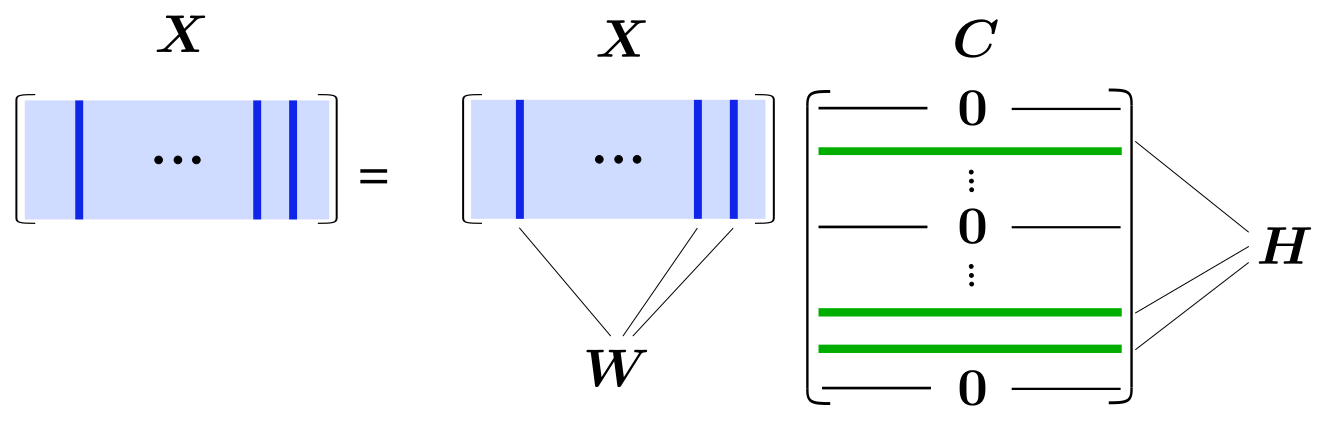
\includegraphics[width=0.7\textwidth]{figures/sdmmv_demo/demo.png}
    %     \caption*{Row-sparsity matrix $\bm{C}_{\text{opt}}$ }
    % \end{figure}

\begin{figure}[ht]
    \centering
    \incfig[0.9]{demoooo}
    \caption*{Row-sparsity matrix $\bm{C}_{\text{opt}}$ }
    \label{fig:demoooo}
\end{figure}

    \note{
    \begin{itemize}
        \item There have been many formulations developed for problem of finding $\mathcal{K}$ under separability condition. One interesting perspective is from self-diction and sparse regression, as shown in this formulation. The objective function is row-0 norm, which counts number of nonzero rows in $\bm{C}$.
        \item The optimal solution of this problem has a particular structure, which is:
            \begin{itemize}
                \item A subset of rows of $\bm{C}$ with indices from $\mathcal{K}$ is $\bm{H}$
                \item The other rows are $ \bm{0}$ rows.
            \end{itemize}
            First of all, [look at picture], we can see that this $\bm{C}$ satisfies all constraints. Objective value at $\bm{C}$ is $K$.
        \item And for a full rank $\bm{W}$, one will need at least $K$ non-zero rows from $\bm{C}$.
        \item With this structure of $\bm{C}_{\text{opt}}$, we can easily identify $\mathcal{K}$.
    \end{itemize}}
\end{frame}

% \begin{frame}
%     \frametitle{demo}
%     \begin{figure}
%         \centering
%         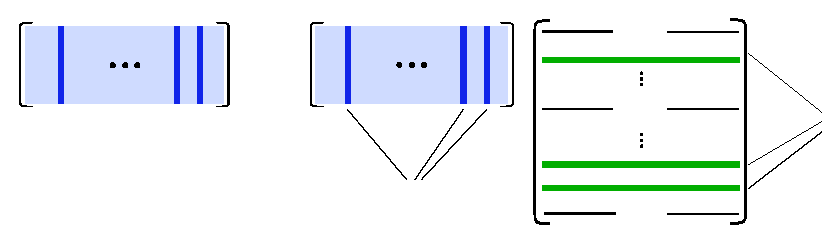
\includegraphics[width=\textwidth]{figures/sdmmv_demo/demonstration.eps}
%     \end{figure}
%     
% \begin{figure}[ht]
%     \centering
%     \incfig{demoooo}
%     \caption{demoooo}
%     \label{fig:demoooo}
% \end{figure}
%
% \end{frame}

% \begin{frame}
%     \frametitle{A Self-Dictionary Perspective}
%     \begin{figure}[t]
%         \begin{subfigure}[b]{0.3\textwidth}
%         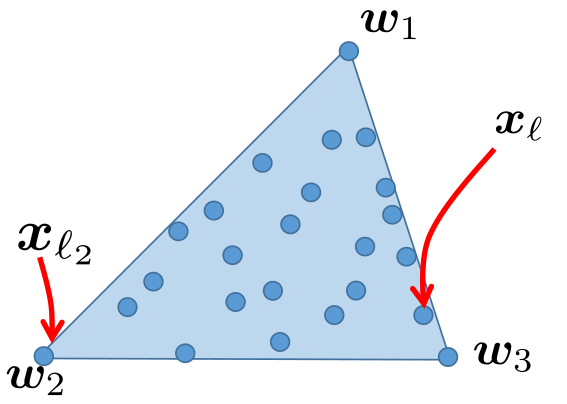
\includegraphics[width=\textwidth]{figures/sdmmv_geometry.png}
%         \caption*{$\bm{x}_\ell = \bm{W}\bm{h}_{\ell}$ \citep{fu2018nonnegative}}
%
%         \end{subfigure}
%         \quad \quad 
%         \begin{subfigure}[b]{0.55\textwidth}
%             \centering
%             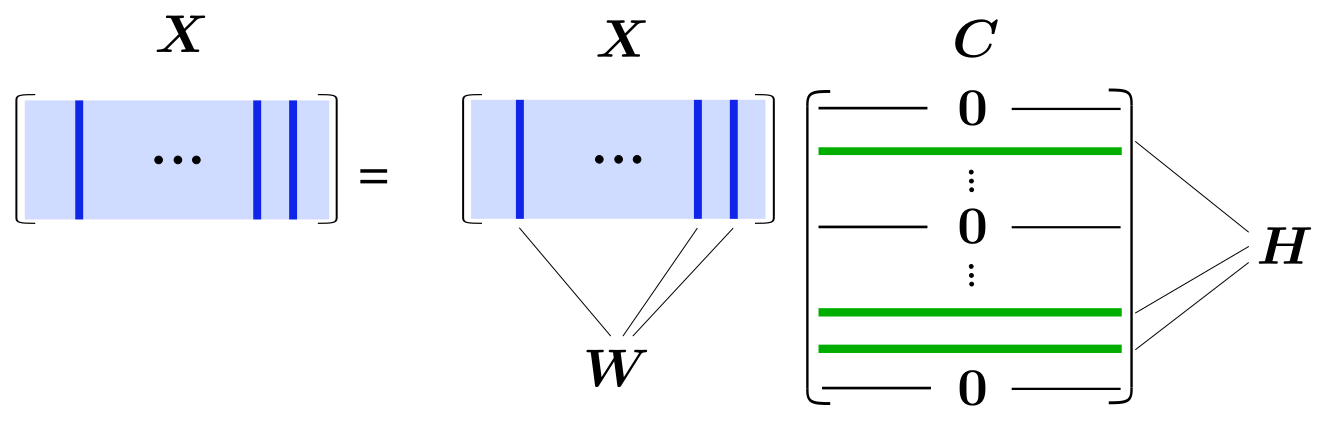
\includegraphics[width=\textwidth]{figures/sdmmv_demo/demo.png}
%             \caption*{Row-sparsity matrix $\bm{C}$ }
%         \end{subfigure}
%     \end{figure}
%     \begin{itemize}
%         \item Since $\bm{h}_\ell \geq 0, \bm{1}^{\T}\bm{h}_\ell=1$, then $\bm{x}_\ell \in \text{conv}(\bm{W})$
%         \item By separability assumption, there exist data points $\bm{x}_\ell$'s at the vertices of $\text{conv}(\bm{W})$
%         \item Hence, each column $\bm{x}_\ell$ is a convex combination of a small subset of columns in $\bm{X}$
% \item Self-dictionary with encouraging row-sparsity 
%     \end{itemize}
%     \begin{alignat*}{2}
%         & \minimize_{\bm{C}} \quad && \norm{\bm{C}}_{\text{row-}0} \\
%         & \text{\rm subject to} && \bm{X} = \bm{X} \bm{C} \\
%         &&& \bm{C} \geq 0, \bm{1}^{\T}\bm{C} = \bm{1}^{\T}
%     \end{alignat*}
%
%     % todo: change layout  to  | text | figure |
%
%     \note{
%     \begin{itemize}
%         \item We are looking for a basis in $\bm{X}$ to represent all columns in $\bm{X}$
%         \item To have a better look at this formulation, or how solving this formulation leads to $\mathcal{K}$? Next slide
%     \end{itemize}}
% \end{frame}

% \begin{frame}
%     \frametitle{A Self-Dictionary Perspective}
%     \begin{itemize}
%         \item Since columns of $\bm{H}$ belongs to a simplex, each column in $\bm{X}$ is a convex combination of $K$ columns of $\bm{W}$
%         \item By separability assumption, and assume that $\mathcal{K} = \set{1, 2, \ldots, N}$
%     \[
%     \bm{X} = \bm{W} \bm{H} = \bm{W} [\bm{I}, \bm{H}'] = [\bm{W}, \bm{W}\bm{H}']
%     \] 
% \item Hence, each column of $\bm{X}$ is a convex combination of a small subset of columns in  $\bm{X}$
% \item Self-dictionary with encouraging row-sparsity 
%     \end{itemize}
%     \begin{columns}
%         \begin{column}{0.3\textwidth}
%     \begin{alignat*}{2}
%         & \minimize_{\bm{C}} \quad && \norm{\bm{C}}_{\text{row-}0} \\
%         & \text{subject to} && \bm{X} = \bm{X} \bm{C} \\
%         &&& \bm{C} \geq 0, \bm{1}^{\T}\bm{C} = \bm{1}^{\T}
%     \end{alignat*}
%         \end{column}
%         \begin{column}{0.7\textwidth}
%             % \begin{figure}[t]
%             %     \centering
%             %     \def\svgwidth{\linewidth}
%             %     \import{./figures/sdmmv_demo}{demonstration.pdf_tex}
%             % \end{figure}
%         \end{column}
%     \end{columns}
%
%     \note{
%     \begin{itemize}
%         \item We are looking for a basis in $\bm{X}$ to represent all columns in $\bm{X}$
%         \item To have a better look at this formulation, or how solving this formulation leads to $\mathcal{K}$? Next slide
%     \end{itemize}}
% \end{frame}


\subsection{Greedy Approach}%
\label{sub:greedy_approach}



\begin{frame}
    \frametitle{Greedy Approach}
    \begin{alignat*}{2}
        & \minimize_{\bm{C}} \quad && \norm{\bm{C}}_{\text{row-}0} \\
        & \text{\rm subject to} && \bm{X} = \bm{X} \bm{C} \\
        &&& \bm{C} \geq 0, \bm{1}^{\T}\bm{C} = \bm{1}^{\T}
    \end{alignat*}
     \begin{itemize}
         \item The greedy approach identifies the set $\mathcal{K}$ by adding one index at a time \citep{fu2014self}.
         \item Successive projection algorithm (SPA) \citep{MC01} is a representative. 
         \item Extracting $\mathcal{K}$ is guaranteed even in noisy case \citep{gillis2014fast}.
         \item All greedy-based methods have a Gram-Schmidt structure which is prone to error propagation under noisy conditions.
     \end{itemize}
     \note{
\begin{itemize}
    % \item Under this the formulation, there are 2 main approaches in the literature.
    \item Solving this optimization problem is not a trivial task. It is firstly not a convex problem due to the row-0, and secondly, and it is a combinatorial problem in essence. 
        % So a native greedy search would be prohibited even if number of vertices $K$ is given.
        \item One of the approaches has been largely studied is greedy approach. As the name suggested, methods in this approach construct set $\mathcal{K}$ by adding 1 index at a time.
        \item A famous successive projection algorithm (SPA) is a representative of this approach.
        \item And it has been shown that estimating exact $\mathcal{K}$ is guaranteed, even under noisy condition.
        \item However, all methods following the greedy approach have a Gram-Schmidt structure in their algorithms. When noise is present, an error made in one iteration will be propagated to future iterations. 
            % This make methods under this approach sensitive to noise.
\end{itemize}
     }
\end{frame}

\subsection{Convex Relaxation Approach}%
\label{sub:convex_relaxation_approach}


\begin{frame}
    \frametitle{Convex Relaxation Approach}
    \begin{itemize}
        \item Relax the problem to a convex optimization problem \citep{gillis2018afast,gillis2014robust,gillis2013robustness,recht2012factoring,Elhamifar2012,Ammanouil2014blind}
        \item An example of this approach is \citep{esser2012convex,fu2015robust,gillis2018afast}
    \begin{alignat*}{2}
        & \minimize_{\bm{C}} \quad && \dfrac{1}{2} \norm{\bm{X} - \bm{X}\bm{C}}_{\rm F}^2 + \lambda R(\bm{C}) \\
        & \text{\rm subject to} && \bm{C} \geq 0, \bm{1}^{\T}\bm{C} = \bm{1}^{\T}
    \end{alignat*}
    where $R(\bm{C})$ is some regularization term to promote row-sparsity.
    % , e.g., 
    % \begin{itemize}
    %     \item \texttt{FastGradient} \citep{gillis2018afast}, $R(\bm{C}) = p^{\T} \text{diag}(\bm{C})$
    % \end{itemize}
    % $\norm{\bm{C}}_{\infty, 1} := \sum^{N}_{n=1} \norm{\bm{C}(n, :)}_{\infty}$.
\item $\mathcal{K}$ is identified in noisy conditions.
\item Often more robust than greedy approach.
    \end{itemize}

    \begin{columns}
        \begin{column}{0.6\textwidth}
         % However, this approach suffers from large memory consumption   
        \begin{alertblock}{Potential Memory Issue}
            The variable $\bm{C}$ has size $N \times N$.
        \end{alertblock}
        A dense matrix $\bm{C}$ with $N=100000$ requires  $74.5$GB.

        
        \end{column}
        \begin{column}{0.5\textwidth}
    \begin{figure}
        \begin{subfigure}{\textwidth}
        \begin{tikzpicture}[scale=0.48]
            \begin{axis}[
                /pgf/number format/1000 sep={},
                xlabel=$N$,
                ylabel=Memory cost in RSS (GB),
                legend pos=north west,
                legend cell align={left},
                xticklabel style={
                        /pgf/number format/fixed,
                },
                scaled x ticks=false,
                % yticklabels={0, 1, 2, 3, 4, 5},
                extra y ticks={1, 3, 5, 6},
                % extra y tick labels={0.3, 5.0},
                % extra tick style={tickwidth=\pgfkeysvalueof{/pgfplots/minor tick length}},
                ]
            \addplot+[red,mark=*,only marks,mark size=3.5pt,mark options={fill=red!50!white}] 
                table [x=N, y=FG]{figures/synthetic_data/exp2/mem.dat};
            \addplot+[dashed,blue,domain=1000:10000, samples=5,mark=none] {0.000000055*x^2 - 0.000024*x + 0.12};
            \legend{\texttt{FastGradient}, curve $aN^2 + b N +c$}
            \end{axis}
        \end{tikzpicture}
        \vspace{-0.25cm}
        \caption*{Memory consumption of \texttt{FastGradient} {\footnotesize \citep{gillis2018afast}}}
        \end{subfigure}
    \end{figure}
        \end{column}
    \end{columns}

    \note{
    \begin{itemize}
        \item The second approach is called convex relaxation.
        \item As mentioned before, the original problem is non-convex, which makes it hard in terms of optimisation. So a natural thing to do is to use a convex opt problem as a surrogate. There has been many convex relaxation formulations proposed in the literature. 
        
            One example is this formulation where the objective function comprises of 2 terms: the fitting error and a regularization to promote row-sparsity of $\bm{C}$.
        \item Under this formulation, identifiability is guaranteed.
        \item Since the algorithm does not suffer from error propagation, it is often more robust then the previous approach. We'll see some evidence on this in our experiments.
        \item However, memory is an obstacle for this approach. Size of variable $\bm{C}$ is $N$ by $N$.  If it is a dense matrix, memory requirement will grow quadratically.  

            As an example, FastGradient is a method following this approach and is considered as state-of-the-art. We run FastGradient on  synthetic data and measure its memory consumption. We can see that memory cost grows quadratically to $N$. This memory cost prohibits this approach's applicability to large scale problem when $N$ could reach to 100000.
        \item The question is can we do any better?
    \end{itemize}
    }
\end{frame}

\section{Proposal: Frank-Wolfe}%
\label{sec:what_are_we_proposing_}

\begin{frame}
    \frametitle{Proposal: Frank-Wolfe}
    In order to gain noise robustness and memory efficiency while obtaining identifiability,
    \begin{itemize}
        \item We follow the convex relaxation approach.
        \item We propose to use Frank-Wolfe as the optimization method to guarantee  $O(KN)$ memory consumption.
    \end{itemize}
    \note{
        Yes, in the followings, I'll present our proposal on the use of FW. Particularly, 
    \begin{itemize}
    \item We follow the convex relaxation approach because of its noise robustness
    \item We propose using Frank-Wolfe method as the optimization method that can guarantee a memory cost of $O(KN)$.
    \end{itemize}
    }
\end{frame}

\subsection{Warm-up: Noiseless Case}%


\begin{frame}
    \frametitle{Warm-up with the Noiseless Case}
% We propose to use Frank-Wolfe as the method to work on convex relaxation formulation.
% For a noiseless case,
    \begin{subequations}
    \label{problem:noiseless_warmup}
    \begin{alignat}{2}
        & \minimize_{\bm{C}} \quad && \dfrac{1}{2} \norm{\bm{X} - \bm{X}\bm{C}}_{\rm F}^2  \\
        & \text{\rm subject to} && \bm{C} \geq 0, \bm{1}^{\T}\bm{C} = \bm{1}^{\T}
    \end{alignat}
    \end{subequations}
    Problem \eqref{problem:noiseless_warmup} can have several solutions
    \begin{itemize}
        \item A desired solution $\bm{C}^{\star}(\mathcal{K}, :) = \bm{H}, \bm{C}^{\star}(\mathcal{K}^{c}, :) = \bm{0}$
        \item A trivial solution $\bm{I}_{N}$
    \end{itemize}

    \begin{figure}[!t]
      \centering
      \hspace{-0.5cm}
      \begin{subfigure}[t]{0.32\textwidth}
      \centering
      \begin{tikzpicture}[scale=0.4]
          \begin{axis}[
              /pgf/number format/.cd,
              1000 sep={},
              xlabel=$n$,
              ylabel=$\norm{\bm{C}_{\text{opt}}(n, :)}_{\infty}$,
              legend pos=south east,
              legend cell align={left},
              ]
          \addplot+[only marks, mark=o, mark size=3.5pt]
              table [x=index, y=norm]{code/pgd_C.dat};
          \addplot+[ycomb, mark=square*, mark size=4pt]
              table [x=index, y=norm]{code/pgd_C_pure_pixel.dat};
          \legend{$n \notin \mathcal{K}$, $n \in \mathcal{K}$}
          \end{axis}
      \end{tikzpicture}
      \caption*{\texttt{APG - Objective value: $3.99{e-}5$}}
      \end{subfigure}
      \begin{subfigure}[t]{0.32\textwidth}
      \centering
      \begin{tikzpicture}[scale=0.4]
          \begin{axis}[
              /pgf/number format/.cd,
              1000 sep={},
              xlabel=$n$,
              ylabel=$\norm{\bm{C}_{\text{opt}}(n, :)}_{\infty}$,
              legend pos=south east,
              legend cell align={left},
              ]
          \addplot+[only marks, mark=o, mark size=3.5pt,] 
              table [x=index, y=norm]{code/fw_C.dat};
          \addplot+[ ycomb, mark=square*, mark size=4pt] 
              table [x=index, y=norm]{code/fw_C_pure_pixel.dat};
          \legend{$n \notin \mathcal{K}$, $n \in \mathcal{K}$}
          \end{axis}
      \end{tikzpicture}

      \caption*{\texttt{FW} - Objective value: $2.86{e-}5$}
      \end{subfigure}
      \begin{subfigure}[t]{0.33\textwidth}
      \centering
      \begin{tikzpicture}[scale=0.4]
          \begin{axis}[
              /pgf/number format/.cd,
              1000 sep={},
              xlabel=iter,
              ylabel=$\text{nnz}(\bm{C}$),
              legend pos=north east,
              legend cell align={left},
              y label style={at={(axis description cs:-0.00,.5)},anchor=south},
              ]
          \addplot[orange,style=very thick] table [x=iter, y=PGD]{code/nnz_fw_pgd.dat};
          \addplot[blue,style=very thick] table [x=iter, y=FW]{code/nnz_fw_pgd.dat};
          \legend{\texttt{APG}, \texttt{FW}}
          \end{axis}
      \end{tikzpicture}
      \caption*{Number of nonzeros (nnz) of $\bm{C}$}
      \end{subfigure}
      \caption*{\texttt{Accelerated proximal gradient (APG)} vs \texttt{Frank-Wolfe (FW)}. Unlike \texttt{APG}, \texttt{FW} outputs exact $\bm{C}^{\star}$ and keeps $\bm{C}$ sparse during its procedure. $M=10, N=50, K=3$}
  \end{figure}  

  \note{
      \begin{itemize}
          \item To see how FW can realize our goal, let's start with a noiseless case. Consider the following simple optimization problem. This problem is convex, but could have multiple solutions.
          \item As example a solution $\bm{C}^{\star}$. It is a desired solution because by inspecting $\bm{C}^{\star}$, such as examining l1-norm of of the rows, we can expect that the l1-norm is $1$ if the corresponding index is from  $\mathcal{K}$, 0 otherwise .
          % For $\bm{C}^{\star}$, if an $n \in \mathcal{K}$, then l1 norm of the $n$-th row of  $\bm{C}^{\star}$ should be $1$. This perfectly holds in the optimal solution of FW. 
          \item There are other solutions as well, for example, an identity matrix, but it provides no information about $\mathcal{K}$.
          \item To demonstrate FW's magic, we run Accelerated Proximal Gradient, a typical first order method for constrained optimization problem, and compare it with Frank-Wolfe.
          \item Firstly, both methods converge and gives a good solutions in terms of objective value.
          However, if we look at l1-norm in the optimal solution, only FW reveals perfect $\mathcal{K}$. 
          \item Secondly, and more interestingly, if we take a look at the density of $\bm{C}$ during the optimization produce, we can see that FW consistently keeps $\bm{C}$ being very sparse, compared to APG. This is the key for memory efficiency when using FW.
      \end{itemize}
  }
\end{frame}

% \begin{frame}[label=fine]
%     \frametitle{Proposal: a Frank-Wolfe Approach}
%     \begin{subequations}
%     \label{problem:noiseless0}
%     \begin{alignat}{2}
%         & \minimize_{\bm{C}} \quad && \dfrac{1}{2} \norm{\bm{X} - \bm{X}\bm{C}}_{\rm F}^2  \\
%         & \text{\rm subject to} && \bm{C} \geq 0, \bm{1}^{\T}\bm{C} = \bm{1}^{\T}
%     \end{alignat}
%     \end{subequations}
% \begin{theorem}[Noiseless Case, Memory Efficiency] \label{theorem:noiseless}
%     %todo let the no repeated unit vectors a trap for questions
%     Suppose that 
%     \begin{itemize}
%         \item $\text{rank}(\bm{W})=K$, no repeated unit vectors exist in $\bm{H}$
%         \item The noise is absent (i.e., $\bm{V}=\bm{0}$)
%         \item Define $\bm{q}_\ell^t = \bm{W}^{\T}\bm{W}(\bm{H}\bm{c}_\ell^t - \bm{h}_\ell)$. Assume 
% \begin{align}\label{eq:nodupq}
%  q_{i,\ell}^t - \min_{j} q_{j,\ell}^t \neq 0,~\forall i \neq \argmin_{j} q_{j,\ell}^t,
% \end{align}
%     \end{itemize}
% Then, using FW  with initialization $\bm{C}^0 = \bm{0}$ to solve \eqref{problem:noiseless0} can reveal exact $\mathcal{K}$ using $O(KN)$ memory.
% \end{theorem}
%
% % \begin{block}{Fact}
% %     Condition \eqref{eq:nodupq} is almost guaranteed if $\bm{W}$ is drawn from some joint continuous distribution.
% % \end{block}
%
% \note{
% \begin{itemize}
%     \item Interesting result, 
%     \item Explain 4 assumptions, causally mention the triviality of the last assumption
%     \item Emphasize: get the right solution, while using less memory
%     \item {\blue Question: is using $\bm{C}=\bm{0}$ valid?}
%     \item {\blue check word "almost guarantee", is it the same as $P=1$.}
% \end{itemize}
% }
% \end{frame}


\begin{frame}
    \frametitle{Frank-Wolfe (FW) method \citep{frank1956algorithm}}
    \begin{itemize}
        \item Assume $f(\bm{x})$ is convex and $\mathcal{D}$ is a compact convex constraint 
    \begin{alignat*}{2}
        & \minimize_{\bm{x}} \quad && f(\bm{x}) \\
        & \text{\rm subject to} && \bm{x} \in \mathcal{D}
    \end{alignat*}
        \item FW's standard procedure: at iteration $t$,
        \begin{align}
        &\bm{s}^{t} \leftarrow \argmin_{\bm{s} \in \mathcal{D}} \; \nabla f(\bm{x}^{t})^{\T} \bm{s} \label{eq:fw_general_update}\\
        &\bm{x}^{t+1} \leftarrow \bm{x}^{t} + \alpha^{t} (\bm{s}^{t} - \bm{x}^{t}) , \quad \alpha^{t}=2/(2+t) \nonumber
        \end{align}

        \item For our problem,
            \begin{block}

      When $\mathcal{D} = \set{\bm{x} \in \mathbb{R}^{n} \mid \bm{x} \geq 0, \bm{1}^{\T}\bm{x} = 1}$, solving $\eqref{eq:fw_general_update}$ only cost $O(n)$, i.e.,          
    \[
    \bm{s} = \bm{e}_{n^{\star}}, \; n^{\star} = \argmin_{n} [\nabla f(\bm{x}^{t})]_n
    \] 
            \end{block}
    % \item FW only update $n^{\star}$-th element of $\bm{x}$ per iteration.
    % \item With $\bm{x}^{0} = \bm{0}$, and $n^{\star} \in \mathcal{K}$, then $\text{supp}(\bm{x}^{t})=K$
% \item With an initialization $\bm{x}^{0} = \bm{0}$, Can we show $n^{\star} \in \mathcal{K}$?
    \end{itemize}
    
    \note{
    \begin{itemize}
        \item Before showing how FW produces such result, let's us briefly review about this method. 
        \item The other name is conditional gradient descent, and has been invented in the 1950s.
        \item It solves a constraint optimization where the objective $f$ is convex and the constraint $\mathcal{D}$ is a compact convex set.
        \item A standard update procedure involves 2 steps. The first step involves a sub-problem which can be solved very efficiently for many constraints.
        \item In our case, the constraint is a probability simplex, and solving it only cost $O(n)$ in terms of computation. 

        In detail, the solution $\bm{s}$ for this step is a canonical unit vector, where the index $n^{\star}$ is index of the smallest element of the gradient. This observation plays an important role that leads to memory efficiency.
    \end{itemize}
    }
\end{frame}

% \begin{frame}
%     \frametitle{Revisit Frank-Wolfe}
%     Given a convex function $f$, a compact convex set  $\mathcal{C}$, FW solves 
%     \begin{alignat*}{2}
%         & \minimize_{\bm{x}} \quad &&  f(\bm{x}) \\
%         & \text{subject to} && \bm{x} \in \mathcal{D}
%     \end{alignat*}
%     with update procedure for $t=0, 1, \ldots $
%     \begin{align}
%         &\bm{s} \leftarrow  \min_{\bm{s} \in \mathcal{D}} \nabla f(\bm{x}^{t})^{\T} \bm{s} \\
%         &\bm{x}^{t+1} \leftarrow (1-\alpha^{t})\bm{x}^{t} + \alpha^{t} \bm{s}, \quad \text{for }  \alpha^{t} = \dfrac{2}{2+t}
%     \end{align}
%    \begin{itemize}
%        \item Does not involve a projection to $\mathcal{D}$.
%        \item Convergence rate $O(1/t)$ [x].
%        \item Scalability [x].
%    \end{itemize} 
% \note{\blue This one should be introduced earlier}
% \end{frame}

% \begin{frame}[label=fine]
%     \frametitle{FW in Noiseless Case}
%     \begin{itemize}
%         \item The objective w.r.t $\bm{c}_\ell$ (omitting $\ell$) is
%     $ f(\bm{c}) = \norm{\bm{X} - \bm{X}\bm{c}}_2^2 $
% \item The FW updates: $\bm{c}^{0} =\bm{0}$, for $t=1, 2, \ldots $
%     \begin{align}
%         &\bm{s} \leftarrow  \min_{\bm{s}\geq 0, \bm{1}^{\T}\bm{s}=1} \nabla f(\bm{c}^{t})^{\T} \bm{s} \label{eq:fw_linear} \\
%         &\bm{c}^{t+1} \leftarrow (1-\alpha^{t})\bm{c}^{t} + \alpha^{t} \bm{s}, \quad \text{for }  \alpha^{t} = \dfrac{2}{2+t}
%     \end{align}
% \item Since \eqref{eq:fw_linear} is a linear problem with a simplex constraint,
%     \[
%     \bm{s} = \bm{e}_{n^{\star}},\quad n^{\star} := \argmin_{n} \; [\nabla f(\bm{c}^{t})]_n
%     \] 
%     \end{itemize}
%     {
% \setbeamercolor{block title}{bg=ForestGreen,fg=black}
%     \begin{block}{ }
%     We will show that $n^{\star} \in \mathcal{K}$. And that leads to memory guarantee
%     \[
%         c_{n}^{t} = 0 \quad   \text{if } n \notin \mathcal{K}
%     \] 
%     \end{block}
%     }
%
%     \note{\blue same frame title, consider using title(1), title(2)}
% \end{frame}

\begin{frame}[label=fine]
    \frametitle{FW in the Noiseless Case}
    \begin{itemize}
        \item The original problem can be solved for each column $\bm{c}$ independently.
    \begin{alignat*}{2}
        & \minimize_{\bm{c} \in \mathbb{R}^{N}} \quad && \dfrac{1}{2} \norm{\bm{x} - \bm{X}\bm{c}}_{\rm F}^2 := f(\bm{c}) \\
        & \text{\rm subject to} && \bm{c} \geq 0, \bm{1}^{\T}\bm{c} = 1
    \end{alignat*}
    \item Updating procedure:
    \begin{align*}
    &\bm{s}^{t} \leftarrow \bm{e}_{n^{\star}}, \quad n^{\star} = \argmin_{n} \; [\nabla f(\bm{x}^{t})] \\
    &\bm{c}^{t+1} \leftarrow \bm{c}^{t} + \alpha^{t} (\bm{s}^{t} - \bm{c}^{t}) , \quad \alpha^{t}=2/(2+t) 
    \end{align*}
    % This can be done sequentially column by column, hence the memory cost for executing is $O(N)$.

    \item If FW picks $n^{\star} \in \mathcal{K}$ in all iterations, then with $\bm{c}^{0}=\bm{0}$, 
        \[\text{supp}(\bm{c}^{t}) \subseteq \mathcal{K}\] 
        holds in all iterations $t$ until FW terminates.
    \end{itemize}


    \note{
    \begin{itemize}
        \item Get back to our problem, note that the original problem is decomposible and hence we can solve it for each column of $\bm{C}$ independently. We omit the subscript denoting index of columns for simplification.
        \item The updating procedure is given by these 2 steps.
        \item The key observation is that when initialising $\bm{c}$ at $ \bm{0}$, if $\bm{n}^{\star} \in \mathcal{K}$, then $\text{supp}(\bm{c}^{t}) \subseteq \mathcal{K}$ for all $t$. This implies that most part of $\bm{C}$ are actually just $0$, only  $KN$ elements in  $C$ aren't.
        \item So the magic is the fact that $n^{\star} \in \mathcal{K}$ really holds.
    \end{itemize}
    }
\end{frame}



\begin{frame}[label=fine]
    \frametitle{FW in the Noiseless Case}
    \begin{block}
        
    FW always picks $n^{\star} \in \mathcal{K}$.
    \end{block}
    \begin{itemize}
        \item Gradient
    \begin{equation*}
        \nabla f(\mathbf{c}) 
        = [\bm{h}_1^{\T}\bm{q}, \ldots , \bm{h}_N^{\T}\bm{q}]^{\T}, \quad \bm{q} = \bm{W}^{\T}\bm{W}(\bm{H}\bm{c}-\bm{h})
    \end{equation*}
    \item For $n^{\star} = \argmin_{n} \bm{h}_n^{\T}\bm{q}$, either
    \begin{itemize}
        \item $\bm{h}_{n^{\star}} = \bm{e}_{k^{\star}}$, where $k^{\star} = \argmin_{k \in [K]} q_k$. By definition, $n^{\star} \in \mathcal{K}$.
        \item $\bm{q} = \bm{0} \Rightarrow$ desired solution $\bm{c}^{\star}$  is found because, 
            \[
            \bm{q} = \bm{0} \Leftrightarrow
            \bm{H}\bm{c} = \bm{h} 
            \xLeftrightarrow{\text{assume $\mathcal{K}=[K]$}}
            \begin{bmatrix}
                \bm{I} & \bm{H}'
            \end{bmatrix}  \bm{c} = \bm{h}
            \Leftrightarrow 
            \bm{c} = \begin{bmatrix}
            \bm{h} \\ \bm{0}
            \end{bmatrix} =\bm{c}^{\star}
            \] 
    \end{itemize}
    \end{itemize}

    To sum up, in the noiseless case, with $\bm{c}^{0} = \bm{0}$,
    \begin{itemize}
        \item $\text{supp}(\bm{c}^{t}) \subseteq \mathcal{K}$ for all $t$.
        \item FW terminates when $\bm{c}^{t} = \bm{c}^{\star} = \begin{bmatrix}
        \bm{h} \\ \bm{0}
        \end{bmatrix}$.
    % \item Therefore, FW outputs $\bm{C}_{\text{opt}} = \bm{C}^{\star}$ using only $O(KN)$ memory.
    \end{itemize}
    
Therefore, FW outputs $\bm{C}_{\text{opt}} = \bm{C}^{\star}$ using only $O(KN)$ memory.
    \note{
    \begin{itemize}
        \item Firstly, gradient has this form
        \item Note that we are looking for index of the smallest element. That index is $n^{\star}$ if either
            \begin{itemize}
                \item $\bm{h}_{n^{\star}}$ is some canonical unit vector.
                \item Or $\bm{q} = \bm{0}$. In this case, we can terminate FW since the desired solution is found.
            \end{itemize}
        \item To sum up, what we have shown is that with initialization at $ \bm{0}$, $\text{supp}(\bm{c})$ is always a subset of $\mathcal{K}$, and when FW terminates, we get a desired solution $\bm{c}^{\star}$. Therefore, we can conclude that FW outputs $\bm{C}^{\star}$ using only $O(KN)$ memory.
    \end{itemize}
    }

\end{frame}

% \begin{frame}[label=fine]
%     \frametitle{FW on Noiseless Case}
%     The original problem can be solved for each column $\bm{c}$ independently
%     \begin{alignat*}{2}
%         & \minimize_{\bm{c} \in \mathbb{R}^{N}} \quad && \dfrac{1}{2} \norm{\bm{x} - \bm{X}\bm{c}}_{\rm F}^2 := f(\bm{c}) \\
%         & \text{\rm subject to} && \bm{c} \geq 0, \bm{1}^{\T}\bm{c} = 1
%     \end{alignat*}
%     \begin{block}{Goal}
%         Show that FW produces the desired solution $\bm{c}^{\star}(\mathcal{K}) = \bm{h}, \bm{c}^{\star}(\mathcal{K}^{c})= \bm{0}$ using $O(K)$ memory.
%     \end{block}
%
%     \begin{itemize}
%     \item Initialize $\bm{c}^{0} =\bm{0}$
%     \item  Updating rule
%         \begin{align*}
%         &\bm{s}^{t} = \bm{e}_{n^{\star}}, \; n^{\star} = \argmin_{n} [\nabla f(\bm{c}^{t})]_n \\
%         &\bm{c}^{t+1} \leftarrow \bm{c}^{t} + \alpha^{t} (\bm{s}^{t} - \bm{c}^{t}) , \quad \alpha^{t}=2/(2+t)
%         \end{align*}
%     \item $n^{\star} \in \mathcal{K}$ holds for every steps
%     \item When FW terminates, $\bm{c}_{\text{opt}}(\mathcal{K}^{c}) = \bm{0}, \bm{c}_\text{opt}(\mathcal{K}) = \bm{h}$
%     \end{itemize}
%
%     \note{
%     \begin{itemize}
%         \item Back to our problem, and notice that we can optimize on columns $\bm{c}$ independently.
%         \item We can explain theoretically why FW works perfectly in this case.
%         \item Particularly, we can show that  \ldots  , where $K$ is usually relatively small to  $N, M$.
%         \item Element of $\bm{c}$ are zero unless some indices $n^{\star}$ are picked during the first step.
%     \end{itemize}
%     }
% \end{frame}

% \begin{frame}
%     \frametitle{FW on Noiseless Case}
%     \begin{itemize}
%         \item Gradient
%     \begin{align*}
%         \nabla f(\mathbf{c}) 
%         =\bm{X}^{\T} (\bm{X}\bm{c} -\bm{x}) 
%         = \bm{H}^{\T} \underbrace{\bm{W}^{\T}\bm{W} (\bm{H}\bm{c} - \bm{h}) }_{\bm{q}} 
%         = [\bm{h}_1^{\T}\bm{q}, \ldots , \bm{h}_N^{\T}\bm{q}]^{\T}
%     \end{align*}
%     \item Lower bound
%     \[
%         [\nabla f(\bm{c})]_n =\bm{h}_n^{\T}\bm{q}
%         \geq \left( \min_{j\in[ K]} q_{j} \right)  \sum^{K}_{j=1} h_{j,n} 
%         = \min_{j\in[ K]} q_{j}
%     \]
%     Lower bound is obtained at $n^{\star}$ when either
%     \begin{itemize}
%         \item $\bm{h}_{n^{\star}} = \bm{e}_{k^{\star}}$, where $k^{\star} = \argmin_{k \in [K]} q_k$. By definition, $n^{\star} \in \mathcal{K}$.
%         \item $\bm{q} = \bm{0} \Rightarrow$ optimal solution is found because
%             \[
%             \bm{q} = \bm{0} \Leftrightarrow
%             \bm{H}\bm{c} = \bm{h} \Leftrightarrow \begin{bmatrix}
%                 \bm{I} & \bm{H}'
%             \end{bmatrix}  \bm{c} = \bm{h}
%             \Leftrightarrow \bm{c} = \begin{bmatrix}
%             \bm{h} \\ \bm{0}
%             \end{bmatrix} 
%             \] 
%     \end{itemize}
%     \end{itemize}
% \end{frame}

\begin{frame}
    \frametitle{FW in the Noisy Case}
        
    \begin{itemize}
        % \item When noise is introduced, solution $\bm{C}_{\texttt{opt}}$ would deviate away from $\bm{C}^{\star}$.
        \item In the noisy case, i.e., $\bm{X} = \bm{W}\bm{H} + \bm{V}, \bm{V} \neq \bm{0}$,
  the gradient is
  \[
      \nabla f(\bm{c}) = [\bm{h}_1^{\T}\bm{q}, \ldots , \bm{h}_n^{\T}\bm{q}] + \bm{n}, \quad ( \bm{n} \text{ depends on the noise $\bm{V}$})
  \] 
  then the picked index $n^{\star}$ could be outside of $\mathcal{K}$.
\item FW is no longer guaranteed to output $\bm{C}^{\star}$.
    \end{itemize}

    \begin{figure}[!t]
      \centering
      \begin{subfigure}[t]{0.32\textwidth}
      \centering
      \begin{tikzpicture}[scale=0.4]
          \begin{axis}[
              /pgf/number format/.cd,
              1000 sep={},
              xlabel=$n$,
              ylabel=$\norm{\bm{C}_{\text{opt}}(n, :)}_\infty$,
              legend pos=south east,
              legend cell align={left},
              ]
          \addplot+[only marks, mark=o, mark size=3.5pt,] 
              table [x=index, y=norm]{code/demo2_35_C.dat};
          \addplot+[ycomb, mark=square*, mark size=4pt] 
              table [x=index, y=norm]{code/demo2_35_pure_pixel.dat};
          \legend{$n \notin \mathcal{K}$, $n \in \mathcal{K}$}
          \end{axis}
      \end{tikzpicture}
      \caption*{\texttt{SNR}$=35$dB}
      \end{subfigure}
      \begin{subfigure}[t]{0.32\textwidth}
      \centering
      \begin{tikzpicture}[scale=0.4]
          \begin{axis}[
              /pgf/number format/.cd,
              1000 sep={},
              xlabel=$n$,
              ytick={0, 0.2, 0.4, 0.6, 0.8, 1.00},
              ymax=1,
              ymin=0,
              ylabel=$\norm{\bm{C}_{\text{opt}}(n, :)}_\infty$,
              legend pos=south east,
              legend cell align={left},
              ]
          \addplot+[only marks, mark=o, mark size=3.5pt,] 
              table [x=index, y=norm]{code/demo2_25_C.dat};
          \addplot+[ycomb, mark=square*, mark size=4pt] 
              table [x=index, y=norm]{code/demo2_25_pure_pixel.dat};
          \legend{$n \notin \mathcal{K}$, $n \in \mathcal{K}$}
          \end{axis}
      \end{tikzpicture}
      \caption*{\texttt{SNR}$=25$dB}
      \end{subfigure}
      \begin{subfigure}[t]{0.32\textwidth}
      \centering
      \begin{tikzpicture}[scale=0.4]
          \begin{axis}[
              xlabel=$n$,
              ytick={0, 0.2, 0.4, 0.6, 0.8, 1.00},
              ymax=1,
              ymin=0,
              ylabel=$\norm{\bm{C}_{\text{opt}}(n, :)}_\infty$,
              legend pos=south east,
              legend cell align={left},
              ]
          \addplot+[only marks, mark=o, mark size=3.5pt] 
              table [x=index, y=norm]{code/demo2_15_C.dat};
          \addplot+[ycomb, mark=square*, mark size=4pt] 
              table [x=index, y=norm]{code/demo2_15_pure_pixel.dat};
          \legend{$n \notin \mathcal{K}$, $n \in \mathcal{K}$}
          \end{axis}
      \end{tikzpicture}
      \caption*{\texttt{SNR}$=15$dB}
      \end{subfigure}
      \caption*{$\bm{C}_{\text{opt}}$ obtained by FW; $M=40, N=50, K=10$.}
  \end{figure}  

  \note{
  \begin{itemize}
      \item However, when noise is introduced, the picked index $n^{\star}$ could be outside of $\mathcal{K}$. 
      \item Thus, FW is no longer guaranteed to output $\bm{C}^{\star}$.
      \item As a simple demonstration, we run FW on 3 cases with increasing noise level. It is evident that when noise is large, the solution obtained by FW could not gives us the desired $\bm{C}^{\star}$.
  \end{itemize}
  }
\end{frame}

\subsection{Enhancement in the Noisy Case}%
\begin{frame}[label=fine]
    \frametitle{Enhancement in the Noisy Case}
    \begin{itemize}
        % \item The prior on $\bm{C}^{\star}$ is exploited to enhance performance in noisy case.
        \item Different regularizations have been used to promote row-sparsity \citep{fu2015robust,esser2012convex,gillis2018afast,gillis2014robust,recht2012factoring,Elhamifar2012}. For example, \citep{fu2015robust,esser2012convex} use
\[
\norm{\bm{C}}_{\infty, 1} := \sum^{N}_{i=1} \norm{\bm{C}(i, :)}_{\infty}
\] 
\item FW works best with smooth functions 
    \[
    \varPhi_{\mu}(\bm{C}) = \sum^{N}_{i=1} \varphi_{\mu}(\bm{C}(i, :)) , \quad \varphi_{\mu}(\bm{C}(i, :)) = \mu \log \left( \dfrac{1}{N} \sum^{N}_{j=1} \exp \left(\dfrac{c_{i, j}}{\mu} \right) \right)
    \] 
\item We propose \texttt{MERIT}, a FW-based algorithm for solving:
    \label{problem:noiseless}
    \begin{alignat*}{2}
        & \minimize_{\bm{C}} \quad && \dfrac{1}{2}\norm{\bm{X} - \bm{X}\bm{C}}_{\rm F}^2 + \lambda \varPhi_{\mu}(\bm{C})  \\
        & \text{\rm subject to} && \bm{C} \geq 0, \bm{1}^{\T}\bm{C} = \bm{1}^{\T}
    \end{alignat*}
    \end{itemize}
    % We name \texttt{MERIT} as a FW implementation for this objective function.

    \note{
    \begin{itemize}
        \item In order to deal with noise, it is common to introduce regularizations. In our problem, the prior is row-sparsity of $\bm{C}$. There have been many different regularizations used in the literature to promote row-sparsity of $\bm{C}$
        \item The mixed-norm l1, l-inf is an example.
        \item In terms of optimization, FW works best with a smooth function. Therefore, we propose a smooth function to approximate the mix-norm l1, l-inf.
        \item The hyperparameter $\mu$ controls the accuracy of approximating  l-inf.
        \item To this end, we propose to solve the following problem. The objective includes 2 terms: the fitting error and our smooth regularization.
        \item Given the convex relaxation on the self-dictionary problem with smooth regularization, we propose \texttt{MERIT}, a FW-based algorithm for solving:

    \end{itemize}
    }
\end{frame}

\begin{frame}[label=fine]
    \frametitle{Identifiability}

    \begin{itemize}
        \item With regularization, we can guarantee the extraction of $\mathcal{K}$ exactly in the noisy case under some reasonable assumptions \citep{nguyen2021memory}. 
        \item This result is obtained using a similar idea to \citep{fu2015robust}.
% \begin{align*}
%     \|\bm{C}_{\text{opt}}(n,:)\|_\infty &> 1- \beta, ~ \forall n \in {\mathcal{K}}, \\
%     \|\bm{C}_{\text{opt}}(n,:)\|_\infty &\leq 2\rho\dfrac{N-K}{ \lambda N} \norm{\bm{V}}_{\rm F}^2 + \mu N \log(N) + \beta K ,  ~~\forall n \notin {\cal K}  \\
% &\beta = \dfrac{ \sqrt{4\rho (1-K/N) \norm{\bm{V}}_{\rm F}^2 + 2{ \lambda} K} + 2\delta } { \kappa(\bm{W})(1-d(\bm{H}))} 
% \end{align*}
        \item Any convex optimization method can be used to obtain $\mathcal{K}$ via solution $\bm{C}_{\text{opt}}$.
    \end{itemize}

    \begin{figure}[!t]
      \centering
      \begin{subfigure}[t]{0.32\textwidth}
      \centering
      \hspace{-1cm}
      \begin{tikzpicture}[scale=0.42]
          \begin{axis}[
              /pgf/number format/.cd,
              1000 sep={},
              xlabel=$n$,
              ylabel=$\norm{\bm{C}_{\text{opt}}(n, :)}_\infty$,
              legend pos=south east,
              legend cell align={left},
              ]
          \addplot+[only marks, mark=o, mark size=3.5pt,] 
              table [x=index, y=norm]{code/demo3_fw_C.dat};
          \addplot+[ycomb, mark=*, mark size=3.5pt,] 
              table [x=index, y=norm]{code/demo3_fw_C_pure_pixel.dat};
          \legend{$n \notin \mathcal{K}$, $n \in \mathcal{K}$}
          \end{axis}
      \end{tikzpicture}
      \caption*{\texttt{MERIT} - Objective value: $3.58{e-}01$}
      \end{subfigure}
      \begin{subfigure}[t]{0.33\textwidth}
      \centering
      \begin{tikzpicture}[scale=0.42]
          \begin{axis}[
              /pgf/number format/.cd,
              1000 sep={},
              xlabel=$n$,
              ylabel=$\norm{\bm{C}_{\text{opt}}(n, :)}_\infty$,
              legend pos=south east,
              legend cell align={left},
              ]
          \addplot+[only marks, mark=o, mark size=3.5pt] 
              table [x=index, y=norm]{code/demo3_pgd_C.dat};
          \addplot+[ycomb, mark=*, mark size=3.5pt]
              table [x=index, y=norm]{code/demo3_pgd_C_pure_pixel.dat};
          \legend{$n \notin \mathcal{K}$, $n \in \mathcal{K}$}
          \end{axis}
      \end{tikzpicture}
      \caption*{\texttt{APG} - Objective value: $4.41{e-}01$}
      \end{subfigure}
      \begin{subfigure}[t]{0.32\textwidth}
      \centering
      \begin{tikzpicture}[scale=0.42]
          \begin{axis}[
              /pgf/number format/.cd,
              1000 sep={},
              xlabel=iter,
              ylabel=$\text{nnz}(\bm{C})$,
              legend pos=south east,
              legend cell align={left},
              y label style={at={(axis description cs:-0.00,.5)},anchor=south},
              ]
          \addplot[orange,style=very thick] table [x=iter, y=FW]{code/demo3_nnz_fw_pgd.dat};
          \addplot[blue,style=very thick] table [x=iter, y=PGD]{code/demo3_nnz_fw_pgd.dat};
          \legend{\texttt{MERIT}, \texttt{APG}}
          \end{axis}
      \end{tikzpicture}
      \caption*{Number of nonzeros (nnz) of $\bm{C}$}
      \end{subfigure}
      \vspace{-0.3cm}
      \caption*{$M=40, K=10, N=50, \texttt{SNR}=30\text{dB}, \mu=1{e-}6, \lambda = 0.1$.}
  \end{figure}
 

  \note{
  \begin{itemize}
      \item We first achieve identifiability when working on this formulation. The result uses a similar idea to this work. 
          % This basically says that using an approximate doesn't break identifiability.
      \item Secondly, it's worth to stress that any convex method can be used to archive identifiability. 
      \item To demonstrate, we run APG and FW on this problem. Both method produce similar optimal objective values, can both optimal solutions can be used to identify $\mathcal{K}$. 
      \item However, it is noticeable that  our method, MERIT, constantly keeps $\bm{C}$ being much more sparse compared to APG. That sparsity is the key of FW's memory efficiency.
  \end{itemize}
  }
\end{frame}
% \begin{theorem}[Identifiability]
%     \label{theorem:identifibility}
% Assume that 
% \begin{itemize}
%     \item $\text{rank}(\bm{W})=K$, no repeated unit vector in $\bm{H}$
%     \item $ \norm{\bm{v}_i}^2 \leq (\rho / N) \norm{\bm{V}}_{\rm F}^2$ for some $\rho$ and  $\norm{\bm{v}_i}_2 \leq \delta$
% \end{itemize}
% Then, any optimal solution $\bm{C}_{\rm opt}$ satisfies: 
% \begin{align*} 
%     \|\bm{C}_{\rm opt}(n,:)\|_\infty &> 1- \highlight{\beta}, ~ \forall n \in {\mathcal{K}}, \\
%     \|\bm{C}_{\rm opt}(n,:)\|_\infty &\leq 2\rho\dfrac{N-K}{ \higreen{\lambda} N} \norm{\bm{V}}_{\rm F}^2 + \higreen{\mu} N \log(N) + \highlight{\beta} K ,  ~~\forall n \notin {\cal K} \nonumber
% \end{align*}
% where 
% \begin{align*}
% &\beta = \dfrac{ \sqrt{4\rho (1-K/N) \norm{\bm{V}}_{\rm F}^2 + 2{ \lambda} K} + 2\delta } { \kappa(\bm{W})(1-d(\bm{H}))} 
% \end{align*} 
% \end{theorem}

% \begin{frame}
%     \frametitle{Identifiability}
%     From the previous,
%     \[
%     \beta = \dfrac{ \sqrt{4\rho (1-K/N) \norm{\bm{V}}_{\rm F}^2 + 2{\lambda} K} + 2\delta } { \kappa(\bm{W})(1-d(\bm{H}))} ,
%     \] 
%     where
% \begin{align*}
% &\kappa(\bm{W}) = \min_{\substack{k \in [K]\\ \bm{1}^{\T}\boldsymbol \theta = 1, \boldsymbol \theta \geq 0}}\; \norm{\bm{w}_k - \bm{W}(:, -k) \boldsymbol \theta}_2^2 \\
% &d(\bm{H}) = \max_{n \in \mathcal{K}, \ell \notin \mathcal{K}} h_{ n, \ell }
% \end{align*} 
% \begin{figure}
%     \centering
%     \begin{subfigure}{0.13\textwidth}
%         \centering
% \begin{tikzpicture}[scale=1.5]
%     \filldraw[color=black, fill=blue!30] (-0.3, 0) -- (0, 1) -- (0.3, 0) -- cycle;
%     \filldraw[color=black, fill=blue!60] (-0.3, 0) circle (0.04);
%     \filldraw[color=black, fill=blue!60] (0, 0.99) circle (0.04);
%     \filldraw[color=black, fill=blue!60] (0.3, 0) circle (0.04);
%
%     \filldraw[color=black, fill=blue!60] (-0.1, 0.3) circle (0.04);
%     \filldraw[color=black, fill=blue!60] (0.01, 0.8) circle (0.04);
%     \filldraw[color=black, fill=blue!60] (0.1, 0.15) circle (0.04);
% \end{tikzpicture}
% \caption*{(1)}
%     \end{subfigure} 
% $<^{\kappa(\bm{W})}$
%     \begin{subfigure}{0.2\textwidth}
%         \centering
% \begin{tikzpicture}[scale=1.5]
%     \filldraw[color=black, fill=blue!30] (-0.6, 0) -- (0, 1) -- (0.6, 0) -- cycle;
%     \filldraw[color=black, fill=blue!60] (-0.6, 0) circle (0.04);
%     \filldraw[color=black, fill=blue!60] (0, 1) circle (0.04);
%     \filldraw[color=black, fill=blue!60] (0.6, 0) circle (0.04);
%
%     \filldraw[color=black, fill=blue!60] (-0.1, 0.3) circle (0.04);
%     \filldraw[color=black, fill=blue!60] (0.01, 0.8) circle (0.04);
%     \filldraw[color=black, fill=blue!60] (0.1, 0.15) circle (0.04);
% \end{tikzpicture}
% \caption*{(2)}
%     \end{subfigure}
%     $<^{d(\bm{H})} \quad$
%     \begin{subfigure}{0.13\textwidth}
%         \centering
% \begin{tikzpicture}[scale=1.5]
%     \filldraw[color=black, fill=blue!30] (-0.6, 0) -- (0, 1) -- (0.6, 0) -- cycle;
%     \filldraw[color=black, fill=blue!60] (-0.6, 0) circle (0.04);
%     \filldraw[color=black, fill=blue!60] (0, 1) circle (0.04);
%     \filldraw[color=black, fill=blue!60] (0.6, 0) circle (0.04);
%
%     \filldraw[color=black, fill=blue!60] (-0.1, 0.3) circle (0.04);
%     \filldraw[color=black, fill=blue!60] (0.01, 0.5) circle (0.04);
%     \filldraw[color=black, fill=blue!60] (0.1, 0.15) circle (0.04);
% \end{tikzpicture}
% \caption*{(3)}
%     \end{subfigure}
%     \caption*{Convex hull of $\bm{W}$. The settings are getting more preferred for identifiability from left to right.}
% \end{figure}
%
%     % However, the theorem does not speak for memory consumption.
% \end{frame}


\begin{frame}
\frametitle{Memory}    
\begin{itemize}
    \item The objective function 
        \[
        h(\bm{C}) = \underbrace{\dfrac{1}{2} \norm{\bm{X} - \bm{X}\bm{C}}_{\rm F}^2}_{f(\bm{C})} + \lambda \varPhi_{\mu}(\bm{C}) = f(\bm{C}) + \lambda \varPhi_{\mu}(\bm{C})
    \]
    \item FW's updating procedure on this problem can be executed column by column sequentially
        % updating procedure of FW of this problem is decomposable so that running it column by column is possible
    % \begin{itemize}
    %     \item Simplex constraint is columns-wise imposed.
    %     \item Linear objective function can be decomposed to columns of $\bm{C}$.
    % \end{itemize}
    \begin{align*}
    &\bm{s}_\ell^{t} \leftarrow \bm{e}_{n^{\star}}, \quad n^{\star} = \argmin_{n} \; [\nabla h(\bm{c}_\ell)]_n  \\
    &\bm{c}_\ell^{t+1} \leftarrow \bm{c}_\ell^{t} + \alpha (\bm{s}_{\ell}^{t}-\bm{c}_{\ell}^{t}), \quad \alpha^{t} = 2/(2+t)
    \end{align*} 
    \item Gradient is given by
\[ 
    \nabla h(\bm{c}_\ell) = \nabla f(\bm{c}_\ell) + \lambda [\nabla \varPhi_{\mu}(\bm{C})]_{:, \ell} 
\] 
%  where
% \[
%     [\nabla \varPhi_{\mu}(\bm{C})]_{n,\ell} = \dfrac{\exp (c_{n, \ell}/\mu)}{\sum^{N}_{i=1} \exp(c_{n, i}/\mu)} 
% \] 
\item Question: If at iteration $t$,  $\text{supp}(\bm{c}_\ell^{t}) \subseteq \mathcal{K}$, can FW pick 
    \[ n^{\star} \in \mathcal{K}, \] where
    $n^{\star} := \argmin_{n}\;[\nabla h(\bm{c}_\ell)]_n$ in iteration $t+1$?
\end{itemize}


\note{
\begin{itemize}
    \item Let's us examine how FW could save memory in this case.
    \item Recall the objective function now includes 2 terms: the fitting error and our regularization term.
    \item Thanks to the updating procedure of FW and also because the constraint being imposing on column-wise, we can perform the update on column by column sequentially. 
        Note that we can run it simultaneously but it would result in $O(N^2)$ memory to store the whole gradient matrix.
    \item The gradient respect to 1 column of $\bm{C}$ is given by this.
    \item The key enables guarantee of memory is that: If at iteration $t$ where we have  $\text{supp}(\bm{c}^{t}) \in \mathcal{K}$, can FW pick $n^{\star} \in \mathcal{K}$ in the next iteration?
    \item Before showing why the statement holds, let's see what is the implication. This statement establishes a recursive relation on $\bm{C}$ between iterations. Hence, if we carefully initilize $\bm{C}$ to construct a base case suth that $\text{supp}(\bm{c}) \in \mathcal{K}$, then the index in next iteration is from $\mathcal{K}$, and hence we also have $\text{supp}(\bm{c}^{t+1}) \in \mathcal{K}$ holds in the next iteration.
That means, the memory cost of saving $\bm{C}$ is again $O(KN)$ as was shown in noiseless case.

    \item Gradient is comprised of 2 terms. Let's us go through these terms.
\end{itemize}
}
\end{frame}


\begin{frame}[label=current]
    \frametitle{Effect of Noise}
\begin{itemize}
    \item Gradient of $f(\bm{c}_\ell) = 1/2\norm{\bm{X} - \bm{X}\bm{C}}_{\rm F}^2$
\begin{align*} 
    &\nabla f(\bm{c}_\ell) = [\bm{h}_1^{\T}\bm{q}_\ell, \ldots , \bm{h}_N^{\T}\bm{q}_\ell]^{\T} + \bm{n}_\ell 
\end{align*}
    \item A demonstration of effect of noise that causes 
        \[
        n^{\star}:=\argmin_{n}\; [\nabla f(\bm{c}_\ell)]_n \notin \mathcal{K}.
    \]
\[
    \footnotesize
\nabla f(\bm{c}_\ell) = 
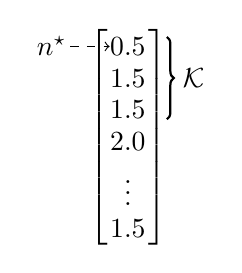
\begin{tikzpicture}[mymatrixenv,baseline=-\the\dimexpr\fontdimen22\textfont2\relax]
    \matrix[mymatrix, ampersand replacement=\&,inner sep=2.5pt,
    % column 1/.style={nodes={fill=blue!10}},
    ] (m)  {
        0.5 \\
        1.5 \\
        1.5 \\
        2.0 \\
        \vdots \\
        1.5 \\
    };
    \node[left=0.5cm of m-1-1, text width=0.3cm] (firstcomm) {$n^{\star}$};
    \mymatrixbraceleft{1}{3}{$\mathcal{K}$};
    \draw[dashed,->] (firstcomm) -- (m-1-1);
    % \node[above=5pt of m-1-1.north west,anchor=south west] (m11) {};
    % \node[above=5pt of m-1-1.north east,anchor=south east] (mm11) {};
    % \fill[myhighlight] 
    %     (m11.south west) -- (m-4-1.north west) -- 
    %     (m-4-1.north east) -- (mm11.south east) -- cycle;
\end{tikzpicture}
 + 
\begin{bmatrix}
0.5 \\
1.5 \\
-0.5 \\
1.0 \\
\vdots  \\
-1.0
\end{bmatrix} 
=
\begin{tikzpicture}[mymatrixenv,baseline=-\the\dimexpr\fontdimen22\textfont2\relax]
    \matrix[mymatrix, ampersand replacement=\&,inner sep=2.5pt,
    % column 1/.style={nodes={fill=blue!10}},
    ] (mx)  {
        1.0 \\
        3.0 \\
        1.0 \\
        3.0 \\
        \vdots  \\
        0.5 \\
    };
    \node[right=0.5cm of mx-6-1, text width=0.3cm] (lastnode) {$n^{\star}$};
    \mymatrixbraceleft{1}{3}{$\mathcal{K}$};
    \draw[dashed,<-] (mx-6-1) -- (lastnode);
\end{tikzpicture}
\]
\end{itemize}

\note {
\begin{itemize}
    \item The first term is gradient of the fitting error. 
    \item Recall that it is a sum of 2 terms:
    \item Because of noise, the smallest element which was shown to be inside of $\mathcal{K}$, now be outside of $\mathcal{K}$.
\end{itemize}
}
\end{frame}

\begin{frame}[label=current]
    \frametitle{Regularization}
    % \begin{block}
    %     
    %     Regularization can ensure $n^{\star} \in \mathcal{K}$ under some reasonable assumptions.
    % \end{block}
    \begin{itemize}
        \item Gradient of the regularization 
\begin{align*} 
    % &\nabla h(\bm{c}_\ell) = [\bm{h}_1^{\T}\bm{q}, \ldots , \bm{h}_N^{\T}\bm{q}]^{\T} + \bm{n}+ \lambda \underbrace{[\nabla \varPhi_{\mu}(\bm{C})]_{:, \ell}}_{\bm{y}_\ell}, 
    &\bm{y}_\ell = [\nabla \varPhi_{\mu}(\bm{C})]_{:, \ell} , \quad 
    y_{n,\ell} = \dfrac{\exp (c_{n, \ell}/\mu)}{\sum^{N}_{i=1} \exp(c_{n, i}/\mu)} 
\end{align*}
        \item Assume that at iteration $t$,  $\text{supp}(\bm{c}^{t}_\ell) \subseteq \mathcal{K}$ for all $\ell$.
\begin{itemize}
    \item For $\; n \notin \mathcal{K}$,
        $ y_{n, \ell} = 1/N$. 
    \item If $\quad \exists n_0 \in \mathcal{K}$ such that $c_{n_0, \ell}$ is not the largest element in row $n_0$ (*), then
    $ y_{n_0, \ell} < \exp ((c_{n_0, \ell} - c_{n_0, \star})/\mu), \quad c_{n_0, \star} = \max_{i} c_{n_0, i} $.
\item (*) can be enforced with some initialization.
\end{itemize}

\item An example of $\bm{C}$ and $\bm{y}_\ell$,
\[
\footnotesize
\bm{C} = 
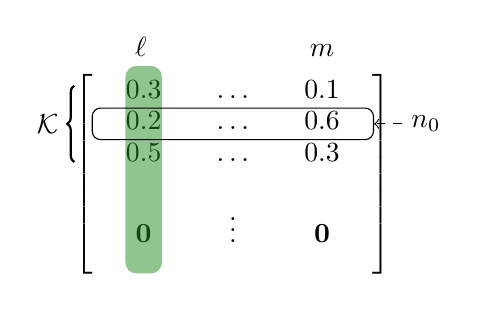
\begin{tikzpicture}[mymatrixenv,baseline=-\the\dimexpr\fontdimen22\textfont2\relax]
    \matrix[mymatrix, ampersand replacement=\&,inner sep=2.5pt,
    ] (m) {
 \vphantom{x} \& 0.3 \& \&\ldots \&   \& 0.1 \& \\
 \vphantom{x} \& 0.2\&\& \ldots \&   \& 0.6 \& \vphantom{x} \\
 \vphantom{x} \& 0.5 \&   \&\ldots\&  \& 0.3 \& \\
 \vphantom{x} \& \vphantom{x} \&\& \& \& \& \\
 \vphantom{x} \&\bm{0} \&\& \vdots \&  \& \bm{0} \& \\
 \vphantom{x} \& \vphantom{x} \&\& \& \& \& \\
    };
    \mymatrixbraceright{1}{3}{$\mathcal{K}$};
    \node[above=5pt of m-1-2.north west, anchor=south west] (l) {$\ell$};
    \node[above=5pt of m-1-2.north east, anchor=south east] (ll) {};
    \node[above=5pt of m-1-6] (m) {$m$};

    \node[below=7em of m-1-2.north west, anchor=north west] (dl) {};
    \node[below=7em of m-1-2.north east, anchor=north east] (dr) {};
    \fill[myhighlight] 
        (l.south west) -- (dl.north west) -- 
        (dr.north east) -- (ll.south east) -- cycle;
    \node[draw,rounded corners=3pt,inner xsep=1pt, fit=(m-2-1)(m-2-7)] (roundk) {};
    \node[right=10pt of roundk] (kkk) {$n_0$};
    \draw[dashed,->] (kkk) -- (roundk);
\end{tikzpicture}
\quad \Longrightarrow \quad
\bm{y}_\ell = 
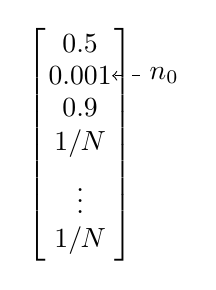
\begin{tikzpicture}[mymatrixenv,baseline=-\the\dimexpr\fontdimen22\textfont2\relax]
    \matrix[mymatrix, ampersand replacement=\&,inner sep=2.5pt,
    ] (y) {
    0.5 \\
    0.001 \\
    0.9 \\
    1/N \\
    \vdots \\
    1/N \\
    };
    \node[right=10pt of y-2-1] (roundk) {$n_0$};
    \draw[dashed,->] (roundk) -- (y-2-1);
\end{tikzpicture}
\] 
    \end{itemize}

    \note{
    \begin{itemize}
        \item The second term is the gradient of regularization.
            % We're considering column $\ell$-th.
        \item Recall that we are assuming that at iteration $t$, we're having a ``good''  $\bm{c}$, in a sense that $\text{supp}(\bm{c}^{t}) $ is a subset of $\mathcal{K}$. 
        \item With such $\bm{c}$, gradient of regularization, which we denote $\bm{y}_\ell$ has a special structure. In particular, 
            \begin{itemize}
                \item For index $n \notin \mathcal{K}$, \ldots 
                \item For index $n_0 $ such that  \ldots 
                \item The existence of $n_0$ can be guarantee by some initialization.
            \end{itemize}

    \end{itemize}
    }
\end{frame}


\begin{frame}[label=current]
    \frametitle{Effect of Regularization}
    \begin{block}

        Regularization can ensure $n^{\star} \in \mathcal{K}$ under some reasonable assumptions.
    \end{block}
    \begin{itemize}
        \item Gradient 
\begin{equation*} 
    \nabla h(\bm{c}_\ell) = \nabla f(\bm{c}_\ell) + \lambda \bm{y}_\ell, 
\end{equation*}
    \item We have 
        \[
            \begin{cases}
                y_{n, \ell} = 1/N \quad & \text{if } n \notin \mathcal{K} \\
                y_{n_0, \ell} \approx 0 \quad& \text{for some }  n_0 \in \mathcal{K}
            \end{cases}
        \] 
        \[
            \Rightarrow n^{\star}:=\argmin_{n} \; [\nabla h(\bm{c}_\ell)]_n = n_0 \quad \text{for some $\lambda$}
        \] 
        % And hence, FW will pick some index $k \in \mathcal{K}$ .
\item An example of $\bm{C}$ and $\nabla h(\bm{c}_\ell)$,
% \[
% \footnotesize
% \bm{C} = 
% \begin{tikzpicture}[mymatrixenv,baseline=-\the\dimexpr\fontdimen22\textfont2\relax]
%     \matrix[mymatrix, ampersand replacement=\&,inner sep=2.5pt,
%     ] (m) {
%  \vphantom{x} \& 0.3 \& \&\ldots \&   \& 0.1 \& \\
%  \vphantom{x} \& 0.2\&\& \ldots \&   \& 0.6 \& \vphantom{x} \\
%  \vphantom{x} \& 0.5 \&   \&\ldots\&  \& 0.3 \& \\
%  \vphantom{x} \&\bm{0} \&\& \vdots \&  \& \bm{0} \& \\
%  \vphantom{x} \& \vphantom{x} \&\& \& \& \& \\
%     };
%     \mymatrixbraceright{1}{3}{$\mathcal{K}$};
%     \node[above=5pt of m-1-2.north west, anchor=south west] (l) {$\ell$};
%     \node[above=5pt of m-1-2.north east, anchor=south east] (ll) {};
%     \node[above=5pt of m-1-6] (m) {$m$};
%
%     \node[below=6em of m-1-2.north west, anchor=north west] (dl) {};
%     \node[below=6em of m-1-2.north east, anchor=north east] (dr) {};
%     \fill[myhighlight] 
%         (l.south west) -- (dl.north west) -- 
%         (dr.north east) -- (ll.south east) -- cycle;
%     \node[draw,rounded corners=3pt,inner xsep=1pt, fit=(m-2-1)(m-2-7)]{};
% \end{tikzpicture}
% \quad \Longrightarrow \quad
% \bm{y}_\ell = 
% \begin{bmatrix}
%     0.5 \\
%     0.001 \\
%     0.9 \\
%     1/N \\
%     \vdots \\
%     1/N
% \end{bmatrix}
% \] 
\[
\footnotesize
\Longrightarrow \nabla h(\bm{c}_\ell) 
=
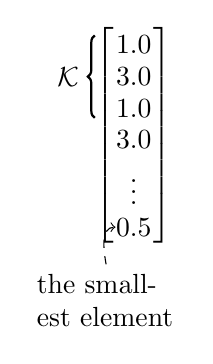
\begin{tikzpicture}[mymatrixenv,baseline=-\the\dimexpr\fontdimen22\textfont2\relax]
    \matrix[mymatrix, ampersand replacement=\&,inner sep=2.5pt,
    ] (m)  {
        1.0 \\
        3.0 \\
        1.0 \\
        3.0 \\
        \vdots  \\
        0.5 \\
    };
    \mymatrixbraceright{1}{3}{$\mathcal{K}$};
    \node[below = 10pt of m-6-1, text width=50pt,xshift=-10pt](smallest) {the smallest element};
    \draw[dashed,->] (smallest.north) to [out=100,in=180] (m-6-1.west);
\end{tikzpicture}
+ 
\lambda
\begin{bmatrix}
    0.5 \\
    0.001 \\
    0.9 \\
    1/N \\
    \vdots \\
    1/N
\end{bmatrix}
\]
    \end{itemize}

    \note{
    \begin{itemize}
        % \item With that, now we can see how regularization can ensure the picked $n^{\star} \in \mathcal{K}$ .
        \item Now we know that the gradient of regularization $\bm{y}_\ell$ has a special structure, such that \ldots 
        \item That would lead to the picked $n^{\star}$ being inside $\mathcal{K}$ for some $\lambda$.

    \end{itemize}
    }
\end{frame}

% \begin{frame}[label=current]
%     \frametitle{Effect of Regularization}
%     % \begin{block}
%     %     
%     %     Regularization can ensure $n^{\star} \in \mathcal{K}$ under some reasonable assumptions.
%     % \end{block}
%     \begin{itemize}
%         \item Gradient of the regularization 
% \begin{align*} 
%     % &\nabla h(\bm{c}_\ell) = [\bm{h}_1^{\T}\bm{q}, \ldots , \bm{h}_N^{\T}\bm{q}]^{\T} + \bm{n}+ \lambda \underbrace{[\nabla \varPhi_{\mu}(\bm{C})]_{:, \ell}}_{\bm{y}_\ell}, 
%     &\bm{y}_\ell = [\nabla \varPhi_{\mu}(\bm{C})]_{:, \ell} , \quad 
%     y_{n,\ell} = \dfrac{\exp (c_{n, \ell}/\mu)}{\sum^{N}_{i=1} \exp(c_{n, i}/\mu)} 
% \end{align*}
% \begin{itemize}
%     \item For $k \notin \mathcal{K}$,
%         $ y_{k, \ell} = 1/N$. 
%     \item If $ \exists k_0 \in \mathcal{K}$ such that $c_{k_0, \ell}$ is not the largest element in row $k_0$ (*), then
%          $ y_{k_0, \ell} < \exp ((c_{k_0, \ell} - c_{k_0, \star})/\mu), \quad c_{k_0, \star} = \max_{i} c_{k_0, i} $ 
%     % \item Therefore, 
%     %     \[
%     %         \begin{cases}
%     %             y_{k_0, \ell} \approx 0 \quad & \\
%     %             y_{k, \ell} = 1/N \quad & \text{if } k \notin \mathcal{K}
%     %         \end{cases}
%     %         \Rightarrow \argmin_{n} \; [\nabla h(\bm{c}_\ell)]_n = k_0 \quad \text{for some $\lambda$}
%     %     \] 
%         % And hence, FW will pick some index $k \in \mathcal{K}$ .
% \end{itemize}
%     % (*) always holds if there exists $k \in \mathcal{K}$ such that $\bm{C}(k, :)$ is not a constant.
%
% \item An example of $\bm{C}$,
% \[
%     \scriptsize
%     \bm{C} = 
% \begin{array}{*7{c}}% matrix for left braces
%     \coolleftbrace{\mathcal{K}}{x \\ x\\ x} \\
%     \vphantom{x} \\
%     \vphantom{x} \\
%     \vphantom{x} \\
% \end{array}%
% \left[  
% \begin{array}{c>{\columncolor{blue!20}}cccccc}
%  & \coolover{\ell}{0.3} & &\ldots &   & \coolover{m}{0.1} & \\
%  \tikzmarkx{left}{\vphantom{0} }&0.2&& \ldots &   & 0.6 &\tikzmarkx{right}{ } \\
%  & 0.5 &   &\ldots&  & 0.3 & \\
%  &\bm{0} && \vdots &  & \bm{0} & \\
%  &&& & & & \\
% \end{array} 
% \right]
% \Highlight[first],
% \quad
% \bm{y}_\ell = 
% \left[
% \begin{array}{c}
%     0.5 \\
%     0.001 \\
%     0.9 \\
%     1/N \\
%     \vdots \\
%     1/N
% \end{array}
% \right]
% \] 
%     \end{itemize}
%
% \end{frame}



\begin{frame}
    \frametitle{\texttt{MERIT} in Noisy Case}
    To sum up, in the noisy case, under some reasonable assumptions, the proposed method \texttt{MERIT} can
    \begin{itemize}
        \item Extract $\mathcal{K}$ exactly.
        \item If $\bm{C}^{t}$ satisfies $\text{supp}(\bm{c}_\ell^{t}) \subseteq \mathcal{K}$ for all $\ell$, then $\text{supp}(\bm{c}_\ell^{t+1}) \subseteq \mathcal{K}$ for all $\ell$, and hence \texttt{MERIT} can guarantee a memory consumption of $O(KN)$.
    \end{itemize}
\end{frame}



\section{Experiment Demonstration}%
\label{sec:real_demonstration}

\subsection{Synthetic Data}%
\label{sub:synthetic}
\begin{frame}
    \frametitle{Synthetic Data}
    \begin{columns}
        \begin{column}{0.5\textwidth}
Data generation
\begin{itemize}
    \item $\bm{W} \sim \mathcal{U}(0, 1)$
    \item $\bm{H} \sim \text{Dir}(\bm{1}), \bm{H}(:, 1:K) = \bm{I}$
    \item $\bm{V} \sim \mathcal{N}(0, \sigma)$
    \item After shuffling $\bm{H}$, $\bm{X} = \bm{W} \bm{H} + \bm{V}$
    \item Noise level is measured in $\texttt{SNR}=10\log_{10} (\sum^{N}_{\ell=1} \norm{\bm{W}\bm{h}_\ell}_2^2)/(MN \sigma^2)$dB
\end{itemize}
Metric
\begin{itemize}
    \item \texttt{success rate} = $P(\mathcal{K} = \widehat{\mathcal{K}})$
    \item Estimate \texttt{success rate} by 50 trials
\end{itemize}
        \end{column}
        \begin{column}{0.65\textwidth}
            \vspace{-0.5cm}
\begin{figure}[!t]
    \centering
    \subfloat[\texttt{success rate} under different SNRs; ${N =200}, M=50, K=40$.]{
    \label{fig:success_rate}
    \centering
    \begin{tikzpicture}[scale=0.48]
        \begin{axis}[
            /pgf/number format/1000 sep={},
            xlabel=\texttt{SNR},
            ylabel=\texttt{success rate},
            legend pos=south east,
            legend cell align={left},
            legend style={at={(0.52,0.01)}, anchor=south west,nodes={scale=0.9}},
            ]
        \addplot[purple,mark=+] table [x=SNR, y=SPA]{figures/synthetic_data/exp1/success_rate.dat};
        \addplot[orange,mark=o] table [x=SNR, y=FG]{figures/synthetic_data/exp1/success_rate.dat};
        \addplot[blue,mark=square] table [x=SNR, y=FW]{figures/synthetic_data/exp1/success_rate.dat};
        \legend{\texttt{SPA}, \texttt{FastGradient}, \texttt{MERIT}}
        \end{axis}
    \end{tikzpicture}
    }

    \subfloat[Memory consumption under different $N$'s;  $\text{SNR}=10\text{dB}, M=50, K=40$.]{
    \label{fig:mem}
    \centering
    \begin{tikzpicture}[scale=0.48]
        \begin{semilogyaxis}[
            /pgf/number format/1000 sep={},
            xlabel=$N$,
            ylabel=Memory cost in RSS (GB),
            legend pos=north west,
            legend cell align={left},
            xticklabel style={
                    /pgf/number format/fixed,
            },
            scaled x ticks=false,
            yticklabels={0., 0.1, 1.0},
            extra y ticks={0.3, 5.0},
            extra y tick labels={0.3, 5.0},
            extra tick style={tickwidth=\pgfkeysvalueof{/pgfplots/minor tick length}},
            ]
        \addplot[orange,mark=o] table [x=N, y=FG]{figures/synthetic_data/exp2/mem.dat};
        \addplot[blue,mark=square] table [x=N, y=FW]{figures/synthetic_data/exp2/mem.dat};
        \legend{\texttt{FastGradient}, \texttt{MERIT}}
        \end{semilogyaxis}
    \end{tikzpicture}
    }
    \caption*{Performance of \texttt{MERIT} compared to baselines}
\end{figure}
            
        \end{column}
    \end{columns}


    \note{
    \begin{itemize}
        \item We first evaluate performance of the proposed method \texttt{MERIT} using synthetic settings.
        \item For identifiability evaluation, we measure the probability of exactly recovering $\mathcal{K}$.
        \item We compare MERIT with other 2 methods: SPA which is a very well-known representative from greedy approach, and FastGradient which is considered state-of-the-art method using convex relaxation approach.
        \item The first figure shows result on success rate. The 2 methods, MERIT and FastGradient are more noise reluctant compared to SPA.
        \item Within MERIT and FastGradient, we also measured their memory consumption. It can be seen in figure b that memory of FastGradient grows much faster compared to MERIT.
    \end{itemize}
    }
\end{frame}

\subsection{Real data}%
\label{sub:real_data}
% \begin{frame}
%     \frametitle{Real Data: Topic Modeling}
%     Metrics:
%     \begin{itemize}
%         \item \texttt{Coherence score} measures the quality of a mined topic. Higher score is better
%         \item \texttt{Similarity count} is measured between topics. Smaller value is better
%         \item \texttt{Accuracy} is measured using topic label. Higher score is better
%     \end{itemize}
%     Data
%     \begin{itemize}
%         \item TDT2
%         \item Reuters-21578 
%     \end{itemize}
% \end{frame}

% \begin{frame}
%     \frametitle{Real Data: Topic Modeling}
% \begin{table}
%     \resizebox{\linewidth}{!}{\small
%     \begin{tabular}{|p{1.2cm}|c|c|c|c|c|c|c|c|c|}
%         \multicolumn{10}{c}{TDT2} \\
%         \hline
%         & \textbf{Method / $K$} & $3$ & $4$ & $5$ & $6$ & $7$ & $8$ & $9$ & $10$ \\
%         \hline
%         \multirow{6}{1.6cm}{Coherence $(\uparrow)$} 
%         & \texttt{SPA} & {\blue -346.6} & -388.4 & -404.9 & -432.0 & -418.6 & -438.2 & -443.5 & -456.7 \\
%         \cline{2-10}
%         & \texttt{FastAnchor} & -468.6 & -483.4 & -483.3 & -495.9 & -525.8 & -536.2 & -546.5 & -543.2 \\
%         \cline{2-10}
%         & \texttt{XRAY} & -347.4 & -389.2 & -405.4 & -432.0 & -419.0 & -439.4 & -443.2 & -459.2 \\
%         \cline{2-10}
%         & \texttt{LDA} & -521.6 & -526.2 & -530.4 & -546.0 & -550.0 & -538.8 & -543.1 & -553.1 \\
%         \cline{2-10}
%         & \texttt{FastGradient} & -553.8 & -517.1 & -537.2 & -534.6 & -561.9 & -562.7 & -571.9 & -585.5 \\
%         \cline{2-10}
%          \rowcolor{green!10} & \texttt{MERIT} & -351.5 & \textbf{-375.7} & \textbf{-385.8} & \textbf{-394.4} & \textbf{-399.3} & \textbf{-417.2} & \textbf{-417.5} & \textbf{-429.1} \\
%         \cline{2-10}
%          % \rowcolor{green!10} & \texttt{MERIT(0)} & \textbf{-345.0} & {\blue -388.4} & {\blue -404.8} & -433.4 & -420.1 & -439.4 & -444.3 & -458.3  \\
%         \hhline{|=|=|=|=|=|=|=|=|=|=|}
%         \multirow{6}{1.6cm}{Similarity Count $(\downarrow)$}
%         & \texttt{SPA} & {\blue 1.06} & 3.64   & 5.76   & 10.24  & 14.24  & 23.18  & 27.56  & 43.62  \\
%         \cline{2-10}
%         & \texttt{FastAnchor} & {\blue 1.06} & \textbf{2.02} & \textbf{3.90} & \textbf{4.80} & \textbf{6.18} & \textbf{7.98} & \textbf{9.92} & \textbf{11.22} \\
%         \cline{2-10}
%         & \texttt{XRAY} & \textbf{1.00} & 3.88 & 5.66 & 10.24& 14.16& 23.18& 28.00& 43.4 \\
%         \cline{2-10}
%         & \texttt{LDA} & 1.08 & {\blue 2.96} & {\blue 5.62} & {\blue 7.84} & {\blue 12.24}& {\blue 17.28}& {\blue 21.84}& {\blue 27.5} \\
%         \cline{2-10}
%         & \texttt{FastGradient} & 14.80 & 26.34 & 47.16 & 62.28 & 71.24 & 100.58& 109.84& 127.32 \\
%         \cline{2-10}
%         \rowcolor{green!10}& \texttt{MERIT} & 1.56 & 4.98 & 5.76 & 7.92 & 13.30 & 21.16 & 28.52 & 36.08 \\
%         \cline{2-10}
%           % \rowcolor{green!10}& \texttt{MERIT(0)} & 1.06 & 3.64 & 5.78 & 10.56 & 14.38 & 22.62 & 27.50 & 43.06 \\
%         \hhline{|=|=|=|=|=|=|=|=|=|=|}
%         \multirow{6}{1.6cm}{Accuracy $(\uparrow)$}
%           & \texttt{SPA} & {\blue 0.87} & {\blue 0.83} & {\blue 0.81} & {\blue 0.81} & {\blue 0.78} & {\blue 0.76} & {\blue 0.75} & {\blue 0.72} \\
%         \cline{2-10}
%         & \texttt{FastAnchor} & 0.77 & 0.72 & 0.67 & 0.63 & 0.66 & 0.63 & 0.65 & 0.65  \\
%         \cline{2-10}
%         & \texttt{XRAY} & {\blue 0.87} & 0.82 & 0.80 & {\blue 0.81} & {\blue 0.78} & {\blue 0.75} & {\blue 0.75} & 0.71 \\
%         \cline{2-10}
%         & \texttt{LDA} & 0.78 & 0.77 & 0.74 & 0.75 & 0.73 & 0.72 & 0.68 & 0.70 \\
%         \cline{2-10}
%         & \texttt{FastGradient} & 0.70 & 0.71 & 0.65 & 0.64 & 0.61 & 0.56 & 0.58 & 0.57 \\
%         \cline{2-10}
%           \rowcolor{green!10} & \texttt{MERIT} & \textbf{0.88} & \textbf{0.88} & \textbf{0.85} & \textbf{0.86} & \textbf{0.84} & \textbf{0.82} & \textbf{0.80} & \textbf{0.77} \\
%          \cline{2-10}
%           % \rowcolor{green!10} & \texttt{MERIT}(0) & 0.86 & {\blue 0.83} & 0.80 & {\blue 0.81} & {\blue 0.78} & {\blue 0.76} & {\blue 0.75} & {\blue 0.72} \\
%         \hline 
%     \end{tabular}}
%     \end{table}
% \end{frame}
\begin{frame}
    \frametitle{Real Data: Topic Modeling}
\begin{table}
    \resizebox{\linewidth}{!}{\small
    \begin{tabular}{|p{1.2cm}|c|c|c|c|c|c|c|c|c|}
        \multicolumn{10}{c}{Accuracy} \\
        \hline
        & \textbf{Method} \textbackslash $K$ & $3$ & $4$ & $5$ & $6$ & $7$ & $8$ & $9$ & $10$ \\
        \hline
        \hhline{|=|=|=|=|=|=|=|=|=|=|}
        \multirow{6}{1.6cm}{TDT2}
          & \texttt{SPA} & {\blue 0.87} & {\blue 0.83} & {\blue 0.81} & {\blue 0.81} & {\blue 0.78} & {\blue 0.76} & {\blue 0.75} & {\blue 0.72} \\
        \cline{2-10}
        & \texttt{FastAnchor} & 0.77 & 0.72 & 0.67 & 0.63 & 0.66 & 0.63 & 0.65 & 0.65  \\
        \cline{2-10}
        & \texttt{XRAY} & {\blue 0.87} & 0.82 & 0.80 & {\blue 0.81} & {\blue 0.78} & {\blue 0.75} & {\blue 0.75} & 0.71 \\
        \cline{2-10}
        & \texttt{LDA} & 0.78 & 0.77 & 0.74 & 0.75 & 0.73 & 0.72 & 0.68 & 0.70 \\
        \cline{2-10}
        & \texttt{FastGradient} & 0.70 & 0.71 & 0.65 & 0.64 & 0.61 & 0.56 & 0.58 & 0.57 \\
        \cline{2-10}
        & \texttt{MERIT} & \textbf{0.88} & \textbf{0.88} & \textbf{0.85} & \textbf{0.86} & \textbf{0.84} & \textbf{0.82} & \textbf{0.80} & \textbf{0.77} \\
        \cline{2-10}
        \hline 
        \multirow{6}{1.6cm}{Reuters-21578}
          & \texttt{SPA} & {\blue 0.64} & 0.57 & {\blue 0.54} & 0.51 & 0.49 & 0.44 & 0.42 & 0.40 \\
        \cline{2-10}
        & \texttt{FastAnchor} & 0.60 & 0.57 & 0.52 & {\blue 0.52} & 0.46 & 0.42 & 0.38 & 0.37 \\
        \cline{2-10}
        & \texttt{XRAY} & 0.63 & 0.57 & {\blue 0.54} & 0.51 & 0.49 & {\blue 0.45} & 0.42 & 0.40 \\
        \cline{2-10}
        & \texttt{LDA} & 0.63 & 0.57 & 0.53 & 0.51 & 0.46 & 0.44 & 0.41 & 0.42 \\
        \cline{2-10}
        & \texttt{FastGradient} & 0.62 & 0.57 & \textbf{0.56} & 0.51 & {\blue 0.50} & \textbf{0.48} & \textbf{0.44} & \textbf{0.46} \\
        \cline{2-10}
        & \texttt{MERIT} & \textbf{0.66} & \textbf{0.62} & 0.53 & \textbf{0.53} & \textbf{0.51} & \textbf{0.48} & {\blue 0.43} & {\blue 0.45} \\
        \hline
    \end{tabular}}
    \caption*{\textbf{Bold}, and {\blue blue} indicate the best and second best scores, resp.}
    \end{table}


    \note{
    \begin{itemize}
        \item In the second experiment, we evaluate MERIT on a topic modeling problem, using 2 real-world datasets: TDT2, Reuters.
        \item Since we have ground truth of topic labels on both dataset, we report Accuracy for performance comparison.
        \item The set of chosen baselines includes several representatives: SPA as a representative of greedy method, FastAnchor, XRAY are variants of SPA developed under topic modeling problem, LDA is a standard baseline for topic modeling. Lastly, FastGradient is method from convex relaxation is included as in the last exp.
        \item MERIT has a consistently good performance in both dataset compared to other baselines.
    \end{itemize}
    }
\end{frame}

% \begin{frame}
%     \frametitle{Real Data: Topic Modeling}
% \begin{table}
%     \resizebox{\linewidth}{!}{\small
%     \begin{tabular}{|p{1.2cm}|c|c|c|c|c|c|c|c|c|}
%         \multicolumn{10}{c}{Reuters-21578} \\
%         \hline
%         & \textbf{Method / $K$} & $3$ & $4$ & $5$ & $6$ & $7$ & $8$ & $9$ & $10$ \\
%         \hline
%         \multirow{6}{1.6cm}{Coherence $(\uparrow)$}
%         & \texttt{SPA} & {\blue -402.7} & -416.4 & \textbf{-420.5} & -442.1 & -516.5 & -520.3 & {\blue -541.5} & {\blue -548.3} \\
%         \cline{2-10}
%         & \texttt{FastAnchor} & -655.0 & -681.0 & -693.6 & -711.1 & - 757.5 & -827.7 & -832.8 & -843.4 \\
%         \cline{2-10}
%         & \texttt{XRAY} & -404.4 & {\blue -415.2} & -422.7 & {\blue -441.6} & {\blue -516.3} & {\blue -519.6} & -542.2 & -548.6 \\
%         \cline{2-10}
%         & \texttt{LDA} & -674.1 & -677.2 & -686.3 & -715.2 & -705.9 & -762.9 & -776.8 & -776.5 \\
%         \cline{2-10}
%         & \texttt{FastGradient} & -657.1 & -768.3 & -782.0 & -821.8 & -847.1 & -967.7 & -989.5 & -959.8 \\
%         \cline{2-10}
%           \rowcolor{green!10}& \texttt{MERIT} & -430.6 & -452.8 & -466.4 & -494.0 & -539.2 & -541.1 & -564.8 & -570.8 \\
%         \cline{2-10}
%         % \rowcolor{green!10}  & \texttt{MERIT(0)} & \textbf{-401.7} & \textbf{-413.3} & {\blue -422.5} & \textbf{-440.8} & \textbf{-511.2} & \textbf{-518.2} & \textbf{-536.0} & \textbf{-544.0} \\
%         \hhline{|=|=|=|=|=|=|=|=|=|=|}
%         \multirow{6}{1.6cm}{Similarity Count $(\downarrow)$}
%         & \texttt{SPA} & 7.46 & 15.16 & 23.82 & 51.98 & 59.38 & 158.50 & 235.62 & 219.16 \\
%         \cline{2-10}
%         & \texttt{FastAnchor} & \textbf{5.40} & {\blue 8.46} & {\blue 13.06} & {\blue 20.06} & {\blue 25.56} & {\blue 42.28} & {\blue 54.9} & {\blue 57.84} \\
%         \cline{2-10}
%         & \texttt{XRAY} & 6.76 & 14.18 & 23.82 & 52.06 & 59.64 & 160.96 & 235.10 & 221.50 \\
%         \cline{2-10}
%         & \texttt{LDA} & \textbf{3.20} & \textbf{6.46} & \textbf{9.32} & \textbf{12.48} & \textbf{21.22} & \textbf{24.60} & \textbf{33.56} & \textbf{39.68} \\
%         \cline{2-10}
%         & \texttt{FastGradient} & 12.96  & 20.62  & 30.42  & 47.56  & 60.46  & 82.86  & 106.66 & 144.38 \\
%         \cline{2-10}
%         \rowcolor{green!10} & \texttt{MERIT} & 7.34 & 16.04 & 21.88 & 36.08 & 48.36 & 93.32 & 131.62 & 141.42 \\
%         \cline{2-10}
%         % \rowcolor{green!10} & \texttt{MERIT(0)} & 7.38 & 15.18 & 23.24 & 45.12 & 54.60 & 145.52 & 223.66 & 214.60 \\
%         \hhline{|=|=|=|=|=|=|=|=|=|=|}
%         \multirow{6}{1.6cm}{Accuracy $(\uparrow)$}
%           & \texttt{SPA} & {\blue 0.64} & 0.57 & {\blue 0.54} & 0.51 & 0.49 & 0.44 & 0.42 & 0.40 \\
%         \cline{2-10}
%         & \texttt{FastAnchor} & 0.60 & 0.57 & 0.52 & {\blue 0.52} & 0.46 & 0.42 & 0.38 & 0.37 \\
%         \cline{2-10}
%         & \texttt{XRAY} & 0.63 & 0.57 & {\blue 0.54} & 0.51 & 0.49 & {\blue 0.45} & 0.42 & 0.40 \\
%         \cline{2-10}
%         & \texttt{LDA} & 0.63 & 0.57 & 0.53 & 0.51 & 0.46 & 0.44 & 0.41 & 0.42 \\
%         \cline{2-10}
%         & \texttt{FastGradient} & 0.62 & 0.57 & \textbf{0.56} & 0.51 & {\blue 0.50} & \textbf{0.48} & \textbf{0.44} & \textbf{0.46} \\
%         \cline{2-10}
%         \rowcolor{green!10}   & \texttt{MERIT} & \textbf{0.66} & \textbf{0.62} & 0.53 & \textbf{0.53} & \textbf{0.51} & \textbf{0.48} & {\blue 0.43} & {\blue 0.45} \\
%         \cline{2-10}
%          % \rowcolor{green!10}  & \texttt{MERIT(0)} & {\blue 0.64} & {\blue 0.58} & {\blue 0.54} & {\blue 0.52} & 0.49 & 0.44 & 0.42 & 0.41 \\
%         \hline 
%     \end{tabular}
% }
%     \end{table}
% \end{frame}
\begin{frame}
    \frametitle{Real Data: Topic Modeling}
% \begin{figure}[t]
%     \centering
%     \subfloat[TDT2] {
%         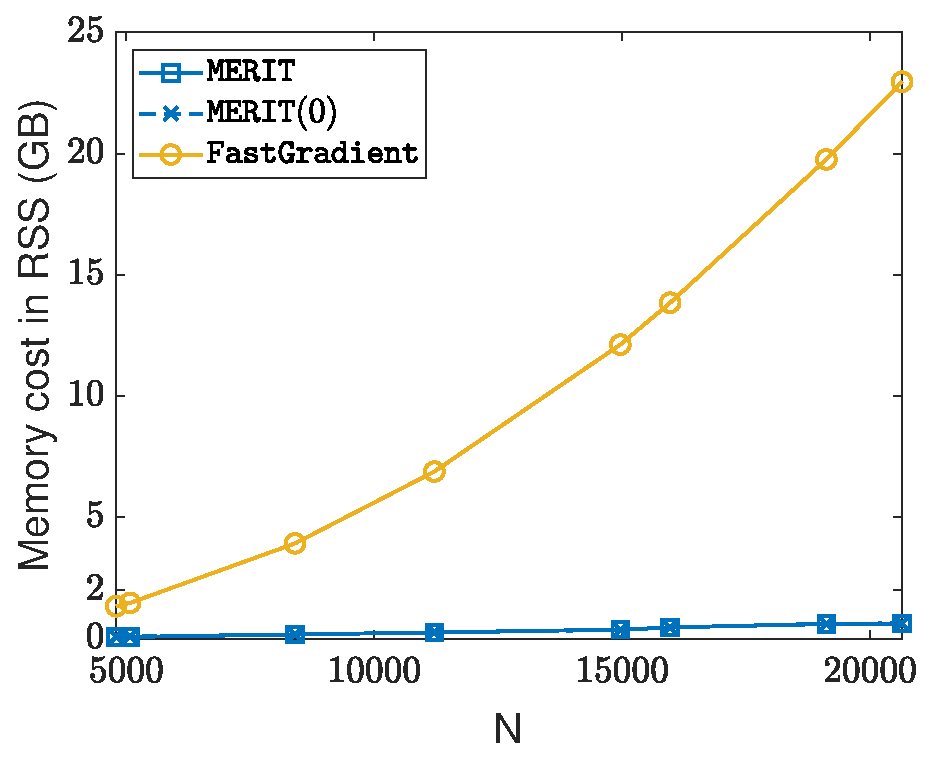
\includegraphics[width=0.35\textwidth]{figures/topic_modeling/tdt2/tdt2_mem.eps}
%         \label{fig:topic_mem_tdt2}
%     }
%     \subfloat[Reuters-21578] {
%         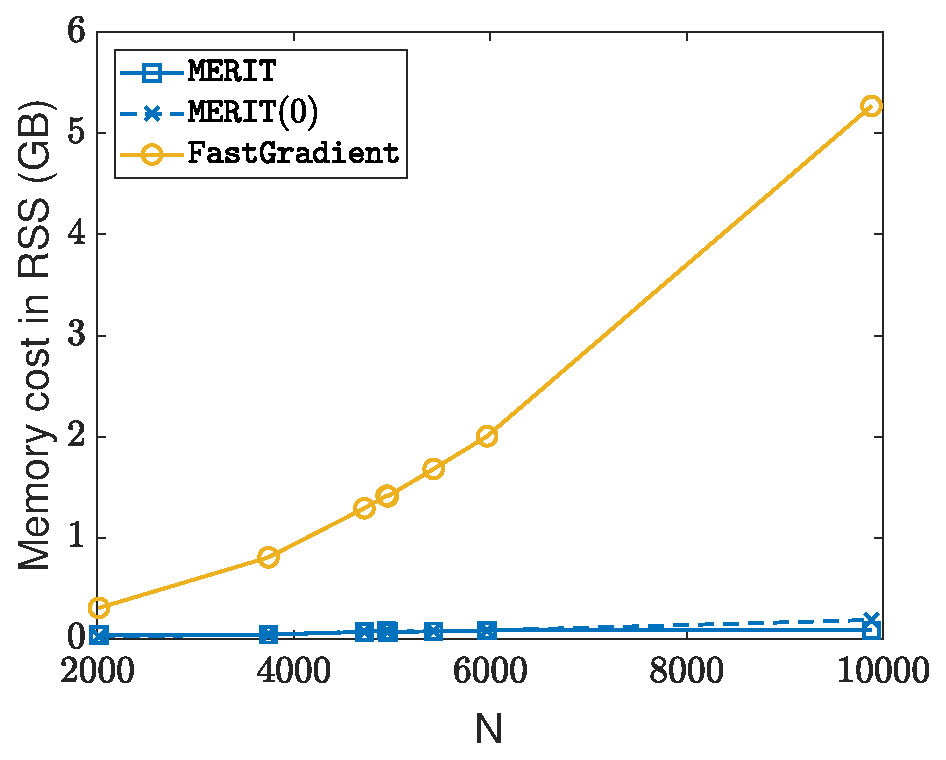
\includegraphics[width=0.35\textwidth]{figures/topic_modeling/reuters/reuters_mem.eps}
%         \label{fig:topic_mem_reuters}
%     }
%     \caption*{Memory consumption of \texttt{FastGradient} and \texttt{MERIT}, under different sample sizes.}
%     \label{fig:topic_mem}
% \end{figure}

\begin{figure}[t]
    \centering
    \begin{subfigure}{0.45\textwidth}
    \begin{tikzpicture}[scale=0.55]
        \begin{axis}[
            /pgf/number format/1000 sep={},
            xlabel=$N$,
            ylabel=Memory cost in RSS (GB),
            legend pos=north west,
            legend cell align={left},
            ]
        \addplot[orange,mark=o] table [x=N, y=FG]{figures/topic_modeling/tdt2/mem.dat};
        \addplot[blue,mark=square] table [x=N, y=FW]{figures/topic_modeling/tdt2/mem.dat};
        \legend{\texttt{FastGradient}, \texttt{MERIT}}
        \end{axis}
    \end{tikzpicture}
    % \captionsetup{justification=centering,margin=0.2cm,font=scriptsize}
    \caption*{TDT2} 
    \end{subfigure}
    \begin{subfigure}{0.45\textwidth}
    \begin{tikzpicture}[scale=0.55]
        \begin{axis}[
            /pgf/number format/1000 sep={},
            xlabel=$N$,
            ylabel=Memory cost in RSS (GB),
            legend pos=north west,
            legend cell align={left},
            ]
        \addplot[orange,mark=o] table [x=N, y=FG]{figures/topic_modeling/reuters/mem.dat};
        \addplot[blue,mark=square] table [x=N, y=FW]{figures/topic_modeling/reuters/mem.dat};
        \legend{\texttt{FastGradient}, \texttt{MERIT}}
        \end{axis}
    \end{tikzpicture}
    \captionsetup{justification=centering,margin=0.2cm,font=scriptsize}
    \caption*{Reuters-21578} 
    \end{subfigure}
    % \captionsetup{justification=centering,margin=0.2cm,font=scriptsize}
    \caption*{Memory consumption of \texttt{FastGradient} and \texttt{MERIT}} 
\end{figure}

\note{
    \begin{itemize}
        \item Moreover, we also measure and compare memory consumption between FastGradient and MERIT. 
        \item Similar observation to the previous exp, amount of memory used by FastGradient is growing much faster than MERIT when $N$ is increasing.
    \end{itemize}
}
\end{frame}

\begin{frame}
    \frametitle{Real Data: Community detection}
    \begin{itemize}
        \item Metric: Spearman's rank correlation (SRC). SRC $\in [-1, 1]$, higher value is better.
        \item Data: co-authorship networks, a community ground truth is defined by
        \begin{itemize}
            \item DBLP:  group of conferences
            \item MAG: ``field of study'' tag
        \end{itemize}
    \end{itemize}
    \begin{columns}
        \begin{column}{0.5\textwidth}
\begin{table}[!t]
    \centering
    \vspace{0.7cm}
        \resizebox{\linewidth}{!}{\large
        \begin{tabular}{|c|c|c|c|c|}
            \hline
            \textbf{Dataset}   &   \texttt{GeoNMF} & \texttt{SPOC} &  \texttt{FastGradient} & \texttt{MERIT}   \\  \hline \hline
            DBLP1 &  0.2974 & {\blue 0.2996} &  \textbf{0.3145} & 0.2937 \\
            DBLP2 &  0.2948 & 0.2126 &  {\blue 0.3237} & \textbf{0.3257}  \\
            DBLP3 &  0.2629 & \textbf{0.2972} &  0.1933 & {\blue 0.2763}  \\
            DBLP4 &  0.2661 & {0.3479} &  0.1601 & \textbf{0.3559}  \\
            DBLP5 &  {\blue 0.1977} & 0.1720 &  0.0912 & \textbf{0.1983}  \\
            MAG1  &  \textbf{0.1349} & {\blue 0.1173} &  0.0441 & 0.1149  \\
            MAG2  & 0.1451& 0.1531 & {\bf 0.2426} & {\blue 0.2414} \\
            \hline
        \end{tabular}}
        % \vspace{0.5cm}
    \caption*{SRC Performance on DBLP and MAG. \textbf{Bold} and {\blue blue} indicate the best and second best scores.}
\end{table}
        \end{column}
        \begin{column}{0.55\textwidth}
\begin{figure}[t]
    \centering
    \vspace{-0.6cm}
    \begin{tikzpicture}[scale=0.55]
        \begin{axis}[
            /pgf/number format/1000 sep={},
            xlabel=$N$,
            ylabel=Memory cost in RSS (GB),
            legend pos=north west,
            legend cell align={left},
            ]
        \addplot[orange,mark=o] table [x=N, y=FG]{figures/community_detection/mem.dat};
        \addplot[blue,mark=square] table [x=N, y=FW]{figures/community_detection/mem.dat};
        \legend{\texttt{FastGradient}, \texttt{MERIT}}
        \end{axis}
    \end{tikzpicture}
    \captionsetup{justification=centering,margin=0.2cm,font=scriptsize}
    \caption*{Memory consumption of \texttt{FastGradient} and \texttt{MERIT}} 
\end{figure}
        \end{column}
    \end{columns}
    
    \note{
        \begin{itemize}
            \item In the last exp, we evaluate MERIT on a community detection problem using 2 common used dataset: BDLP and MAG. 
            \item Since they both provide label on community membership, we compare performance based on SRC. Higher score means a better alignment between prediction and ground truth.
            \item For baseslines, we compare with GeoNMF and SPOC, both are popular greedy method for community detection problem, and FastGradient is also included as before.
            \item As we can see, MERIT has a good performance as it was in top 2 in 5 out of 7 cases.
            \item In terms of memory consumption, we observed a consistent result with previous experiment: FastGradient's memory grows much faster than MERIT.
        \end{itemize}
    }
\end{frame}

\begin{frame}
    \frametitle{Conclusion}
    \begin{itemize}
        % \item Separable NMF has been tacked by 2 main approaches: greedy methods and convex relaxation algorithms
        % \item Greedy methods suffer from error propagation, while convex relaxation algorithms is limited by its huge memory requirement
        \item FW is proposed as a memory efficient method for solving separable simplex-structured matrix factorization via convex relaxation.
            % convex relaxation approach to tackle separable NMF
        \item When noise is absent, using FW can bring identification with memory $O(KN)$
        \item For the noisy case, we have proposed using a smooth regularization to guarantee identifiability.
        \item For the noisy case, we have also shown that running FW only cost $O(KN)$ under some reasonable assumptions.

            % {[\blue \scriptsize T. Nguyen, X. Fu, and R. Wu, ``Memory-efficient convex optimization for self-dictionary separable nonnegative matrix factorization: A Frank-Wolfe approach, '' IEEE TSP, revised. (2nd round revision)]}
    \end{itemize}

    The talk is based on {\scriptsize [\fullcite[IEEE TSP, revised. (2nd round revision)]{nguyen2021memory}.]}
\end{frame}

% \begin{frame}
%     \frametitle{Future Work: Zero-Inflation Community Detection}
%     \begin{align*}
%     &\bm{P} = \bm{M} \bm{B} \bm{M}^{\T} , \\
%     &O_{ij} \sim \text{Bernoulli}(P_{ij}) \\
%     &D_{ij} \sim \text{Bernoulli}(T_{ij}) \\
%     &A_{ij} = \begin{cases}
%         O_{ij} \quad & \text{if } D_{ij} = 1 \\
%         0 & \text{otherwise}
%     \end{cases}
%     \end{align*}
%     Given the observations $A_{ij}, (i,j) \in \Omega$, we hope to estimate $\bm{M}, \bm{B}$.
% \end{frame}
\appendix
\begin{frame}[allowframebreaks]
    \frametitle{Reference}
    { \footnotesize
    \printbibliography}
\end{frame}
\begin{frame}
    \frametitle{Condition (*)}

    \begin{block}{Claim:}
        $ \exists n_0 \in \mathcal{K}$ such that $\bm{C}(n_0, :)$ is not a constant

$\Rightarrow \exists n_0 \in \mathcal{K} $  such that $c_{n_0,\ell}$ is not the largest element in row $n_0$ (*).
    \end{block}


\begin{itemize}
    \item Assume that for all $n \in \mathcal{K}$, $c_{n,\ell}$ is the largest element in row $n$.
    \item Then for row $n_0$ such that  $\bm{C}(n_0, :)$ is not a constant, 
        \[
        \exists m, \quad c_{n_0, \ell} > c_{n_0, m}
        \] 
    \item That leads to
        \[
        1 = \bm{1}^{\T}\bm{c}_{\ell} > \bm{1}^{\T} \bm{c}_m = 1
        \] 
    \item The contradiction concludes our claim.
\end{itemize}
An example of $\bm{C}$,
\[
    \scriptsize
    \bm{C} = 
\begin{array}{*7{c}}% matrix for left braces
    \coolleftbrace{\mathcal{K}}{x \\ x\\ x} \\
    \vphantom{x} \\
    \vphantom{x} \\
    \vphantom{x} \\
\end{array}%
\left[  
\begin{array}{c>{\columncolor{blue!20}}cccccc}
 & \cooloverH{\ell}{\cdot} & &\ldots &   & \cooloverH{m}{\cdot} & \\
 \tikzmarkx{left}{\vphantom{0} }&0.6&& \ldots &   & 0.5 &\tikzmarkx{right}{ } \\
 & \cdot &   &\ldots&  & \cdot & \\
 &\bm{0} && \vdots &  & \bm{0} & \\
 &&& & & & \\
\end{array} 
\right]
\Highlight[first]
\]
\end{frame}

% https://tex.stackexchange.com/questions/332027/how-to-annotate-matrices-with-circles-and-arrows
\end{document}
